%% =========================================================================
%%  Core Signatures and Inversions --- 2026 revision
%%
%%  Self-contained revision of the 2023 LyX-exported source.
%%  Source kept frozen at:  ../2023/CoreSignaturesAndInversions.tex
%%
%%  Major changes vs 2023:
%%    - Introduction cut by ~60% (Toquinho epigraph dropped, related-work
%%      tour compressed, section roadmap removed)
%%    - Section 2: dense sin tables (Tables Levelupto3Sins and Level4Sins
%%      in 2023 source) moved to companion notebook reference
%%    - Section 3: 12 per-level subsubsections collapsed to one worked
%%      level (3) + summary table; structural result via Lyndon /
%%      Witt now leads, Gröbner derivation reframed as constructive
%%      corollary
%%    - Section 4: dense three-piece Chen equation tables moved to
%%      Appendix; new closing subsection on the regression / norm-
%%      equivalence picture
%%    - Section 5 (term structures in finance) dropped; one paragraph
%%      in Conclusions points to forthcoming BRL+USD paper
%%    - Theorem environments declared so the new structural results
%%      appear with proper numbering
%% =========================================================================

\documentclass[12pt,english]{article}
\usepackage[T1]{fontenc}
\usepackage[utf8]{inputenc}
\usepackage[table]{xcolor}
\usepackage{colortbl}
\usepackage{babel}
\usepackage{cprotect}
\usepackage{float}
\usepackage{url}
\usepackage{amsmath}
\usepackage{amssymb}
\usepackage{amsthm}
\usepackage{graphicx}
\usepackage[a4paper]{geometry}
\geometry{verbose,tmargin=3cm,bmargin=3cm,lmargin=2.5cm,rmargin=2.5cm,footskip=1cm}
\usepackage{fancyhdr}
\pagestyle{fancy}
\usepackage[pdfusetitle,
 bookmarks=true,bookmarksnumbered=false,bookmarksopen=false,
 breaklinks=false,pdfborder={0 0 1},backref=false,colorlinks=false]
 {hyperref}
\hypersetup{colorlinks=true,citecolor=blue}

\makeatletter
\providecommand{\tabularnewline}{\\}
\floatstyle{ruled}
\newfloat{algorithm}{tbp}{loa}
\providecommand{\algorithmname}{Algorithm}
\floatname{algorithm}{\protect\algorithmname}
\makeatother

\usepackage{lastpage}
\usepackage{breakcites}
\lhead{}\chead{}\rhead{}
\lfoot{}\cfoot{{Page} \thepage { of} \pageref{LastPage}}\rfoot{}
\renewcommand{\headrulewidth}{0pt}
\usepackage{indentfirst}

\makeatletter
\providecommand*{\shuffle}{\mathbin{\mathpalette\shuffle@{}}}
\newcommand*{\shuffle@}[2]{%
  \sbox0{$#1\vcenter{}$}%
  \kern .15\ht0
  \rlap{\vrule height .25\ht0 depth 0pt width 2.5\ht0}%
  \raise.1\ht0\hbox to 2.5\ht0{%
    \vrule height 1.75\ht0 depth -.1\ht0 width .17\ht0
    \hfill
    \vrule height 1.75\ht0 depth -.1\ht0 width .17\ht0
    \hfill
    \vrule height 1.75\ht0 depth -.1\ht0 width .17\ht0}%
  \kern .15\ht0
}
\makeatother

\usepackage{listings}
\renewcommand{\lstlistingname}{Listing}

%% Filename / path display: xurl allows breaks at any character so long
%% notebook names like CoreSignatures202412.nb can break gracefully in
%% any sentence position. \nbfile{} is the consistent wrapper to use
%% for filenames; if you ever want to change the breaking strategy
%% (e.g. switch back to \texttt or to \seqsplit), edit this one line.
\usepackage{xurl}
\newcommand{\nbfile}[1]{\nolinkurl{#1}}

%% Allow TeX to expand justification in difficult paragraphs (citation-
%% dense lines, long monospace tokens) rather than letting them bleed
%% into the right margin. Tradeoff: text in such paragraphs is slightly
%% looser; in exchange, no visible right-margin overflow.
\setlength{\emergencystretch}{3em}

%% Theorem environments (new in 2026)
\newtheorem{theorem}{Theorem}
\newtheorem{proposition}[theorem]{Proposition}
\newtheorem{corollary}[theorem]{Corollary}
\newtheorem{lemma}[theorem]{Lemma}
\newtheorem{conjecture}[theorem]{Conjecture}
\theoremstyle{remark}
\newtheorem{remark}[theorem]{Remark}

\begin{document}

\title{Core Signatures and Inversions}
\author{Marcos Costa Santos Carreira\thanks{marcoscscarreira@gmail.com}}
\date{\today}
\maketitle

\begin{abstract}
The signature transform of a path produces a feature representation
with several useful invariance and approximation properties, but the
truncated signature is redundant. The standard remedy is the log signature,
which has the dimension of the free nilpotent Lie algebra but is more
expensive to compute. We introduce \emph{core signatures}: subsets
of the truncated signature with the same dimension as the log signature,
identified algorithmically through the shuffle product and identified
structurally with the Lyndon coordinates of the universal step-$n$
free nilpotent Lie group $G^{n}(\mathbb{R}^{d})$. We then use Chen's
identity to invert a core signature into a piecewise linear path of
two, three, or more segments that exactly reproduces the target signature
up to a chosen truncation level, and frame the multi-segment inversion
as a weighted nonlinear least-squares regression in signature space.
We state a precise norm-equivalence conjecture that would identify
this regression with a Sobolev projection on path space, supported
by structural arguments and numerical evidence. Mathematica code and
the latest companion notebook are available at \url{https://github.com/MarcosCarreira/CoreSignatures}.

\medskip{}
\textit{Keywords}: signatures; log signatures; Lyndon words; Witt
formula; signature inversion; rough paths

\pagebreak{}
\end{abstract}

%% =========================================================================
\section{Introduction}
%% =========================================================================

Signatures are the standard feature representation for paths in rough
path theory and in machine-learning applications to time series (\cite{Lyons,Primer,Fermanian_Thesis}).
For a path $X:[a,b]\to\mathbb{R}^{d}$ of bounded variation, the signature
$S(X)_{a,b}$ is the collection of all iterated integrals along $X$;
truncated at level $m$, it provides a finite-dimensional faithful
encoding of $X$ modulo tree-like equivalence. The truncated signature
contains redundancies arising from the shuffle relations, and the
standard tool for stripping them is the log signature, whose dimension
matches that of the free nilpotent Lie algebra $\mathfrak{g}^{m}(\mathbb{R}^{d})$
of step $m$ on $d$ generators (\cite{log signatures,iisignature CRISM,iisignature,iisignature 1004}).

This paper develops two practical results. First, we identify a subset
of the truncated signature --- the \emph{core signature} --- with
the same dimension as the log signature but consisting of actual signature
entries. Once the identification with the Lyndon coordinates of the
free nilpotent Lie group is in place, the core entries are read directly
from $S(X)_{a,b}$ without any change of basis at computation time;
the identification itself rests on Reutenauer's basis theorem for
the free Lie algebra, the Poincaré--Birkhoff--Witt isomorphism, and
Radford's theorem on the shuffle algebra (all classical). The core
elements turn out to be exactly the entries indexed by Lyndon words
on the alphabet $\{1,\ldots,d\}$, and their count is given by Witt's
formula. Second, we use Chen's identity to invert
a core signature into a concatenation of two or three line segments
in the time-ordered case, and into longer concatenations through a
weighted least-squares regression in signature space whose solutions
empirically coincide with the optimal piecewise-linear $L^{1}$ approximation
of the target.

The closest related work is \cite{varieties}, who study the algebraic
geometry of the universal variety $G^{n}(\mathbb{R}^{d})$ and identify
its dimension with the log-signature size, and \cite{learning}, who
study polynomial and piecewise-linear paths up to level three. The
coordinate-theoretic identification of the Lyndon-indexed signature
entries with a transcendence basis of $\mathcal{O}(G^{n}(\mathbb{R}^{d}))$
is classical and follows from Reutenauer and Radford; our contribution
in Section \ref{sec:Core} is therefore the computational packaging
--- naming the subset, exhibiting an explicit shuffle-product elimination
that produces it, tabulating the substitution rules $Q_{m}$, and using
the resulting coordinates for Chen-based inversion --- rather than
a new coordinate theorem. The Gröbner-basis derivation of Section
\ref{sec:Core} is the algorithmic realisation of the abstract identification
with Lyndon coordinates. For inversion algorithms in the smooth-path
regime see \cite{inversion}.

After our 2023 preprint, two computational-algebra developments deserve
mention. \cite{macaulay2} introduce a Macaulay2 package, \texttt{PathSignatures},
that computes signature varieties of piecewise polynomial paths and
explicitly implements the Lyndon-shuffle representation underlying
our substitution rules $Q_{m}$: their method \texttt{lyndonShuffle}
expresses an arbitrary word in $T(\mathbb{R}^{d})$ as a shuffle polynomial
in Lyndon words, which is the same operation our Gröbner-basis derivation
makes constructive. In Section 6 of that paper they use the term \emph{core
signature tensor} with a meaning different from ours: their core tensor
is the signature of a base path $D$ such that the paths of interest
are obtained from $D$ by linear transformations $A\circ D$, parametrising
\emph{families} of signatures through the linear group action. Our
core signature is a subset of the entries of a single signature, addressing
redundancy \emph{within} one path's signature. The two constructions
are complementary rather than competing --- theirs is suited to the
algebraic geometry of signature varieties; ours to Chen-based inversion
of individual signatures --- but the terminology overlap is worth flagging.
A parallel Julia/OSCAR implementation of related computational tools
is described in \cite{signaturetensorsjl}.

%% =========================================================================
\section{Signatures\label{sec:Signatures}}
%% =========================================================================

\subsection{Definitions}

\subsubsection{Paths and iterated integrals}

A \emph{path} is a continuous map $X:[a,b]\to\mathbb{R}^{d}$. Going
forward we assume bounded variation and piecewise differentiability;
the standard reference for the more general theory is \cite{Lyons}.
The interval $[a,b]$ may always be reparametrised to $[0,1]$.

The signature of $X$ is the formal series
\begin{equation}
S(X)_{a,b}\;=\;\Bigl(1,\;S(X)_{a,b}^{i_{1}},\;S(X)_{a,b}^{i_{1},i_{2}},\;\ldots\Bigr)\,,\qquad i_{k}\in\{1,\ldots,d\}\,,
\end{equation}
whose level-$k$ entries are the iterated integrals
\begin{equation}
S(X)_{a,t}^{i_{1},\ldots,i_{k}}\;=\;\int_{a}^{t}\!\int_{a}^{t_{k}}\!\!\cdots\int_{a}^{t_{2}}dX_{t_{1}}^{i_{1}}\,\cdots\,dX_{t_{k}}^{i_{k}}\,.\label{eq:IteratedIntegral}
\end{equation}
We work throughout with truncated signatures and write
$S^{(\leq m)}(X)_{a,b}$ when emphasising the truncation level. The
total number of entries up to level $m$ on a $d$-letter alphabet
is, for $d>1$,
\begin{equation}
\#\{\text{entries up to level }m\}\;=\;\sum_{k=0}^{m}d^{k}\;=\;\frac{d^{m+1}-d}{d-1}\,.\label{eq:SignSize}
\end{equation}

For a single line segment $X(t)=(\alpha_{1}+\beta_{1}t,\ldots,\alpha_{d}+\beta_{d}t)$,
$t\in[a,b]$, the iterated integrals are explicit at all levels:
\begin{equation}
S(X)_{a,b}^{i_{1},\ldots,i_{k}}\;=\;\frac{\beta_{i_{1}}\beta_{i_{2}}\cdots\beta_{i_{k}}\,(b-a)^{k}}{k!}\,.\label{eq:LineSignature}
\end{equation}
This formula makes line segments the natural building blocks for the
inversion of Section \ref{sec:Inversion}.

The Mathematica function \texttt{signat[paths,limits,level]} that
computes \eqref{eq:IteratedIntegral} symbolically is in the companion
notebook \nbfile{CoreSignatures.nb}. Worked signatures of the cubic
$\{t,t^{3}\}$, the unit circle $\{\cos t,\sin t\}$, and the family
$\{t,\sin(k\pi t^{q})\}$ for $k=1,\ldots,3$ and $q=1,2$ --- including
the closed forms in terms of the Fresnel integrals --- are tabulated
in the same notebook.

\subsection{Properties}

\subsubsection{Translation invariance}

The signature \eqref{eq:LineSignature} depends only on the slopes
$\beta_{i}$ and the duration $b-a$, not on the offsets $\alpha_{i}$.
This holds in general: the signature encodes the shape of the path
modulo translation, so the initial value $X_{a}$ must be tracked
separately when needed.

\subsubsection{Shuffle product}

A $(p,q)$-shuffle of two ordered sequences of lengths $p$ and $q$
is an interleaving that preserves the relative order within each sequence.
Writing the shuffle of two multi-indices $I,J$ as $I\shuffle J$
(the multiset of all valid interleavings), the \emph{shuffle product
identity} for any path $X$ states
\begin{equation}
S(X)_{a,b}^{I}\cdot S(X)_{a,b}^{J}\;=\;\sum_{K\in\,I\shuffle J}S(X)_{a,b}^{K}\,.\label{eq:ShuffleProduct}
\end{equation}
Equation \eqref{eq:ShuffleProduct} is the algebraic engine of Section
\ref{sec:Core}: it provides the polynomial relations among signature
entries that allow us to identify a free generating set. The recursive
implementation of $\shuffle$ used in the companion notebook is the
top answer of \href{https://mathematica.stackexchange.com/questions/41614/shuffle-product-of-two-lists}{this Mathematica.SE thread}.

\subsubsection{Chen's identity\label{subsec:ChenIdentity}}

Given consecutive paths $X:[a,b]\to\mathbb{R}^{d}$ and $Y:[b,c]\to\mathbb{R}^{d}$,
the concatenation $Z=X*Y:[a,c]\to\mathbb{R}^{d}$ has signature given
by Chen's identity (\cite{Lyons}):
\begin{equation}
S(Z)_{a,c}\;=\;S(X)_{a,b}\otimes S(Y)_{b,c}\,.\label{eq:ChenIdentity}
\end{equation}
Componentwise, abbreviating $x_{w}=S(X)_{a,b}^{w}$, $y_{w}=S(Y)_{b,c}^{w}$,
$z_{w}=S(Z)_{a,c}^{w}$, with the conventions $x_{\emptyset}=y_{\emptyset}=1$,
\begin{equation}
z_{i_{1},\ldots,i_{k}}\;=\;\sum_{j=0}^{k}x_{i_{1},\ldots,i_{j}}\cdot y_{i_{j+1},\ldots,i_{k}}\,.\label{eq:ChenIndex}
\end{equation}
The convolution form \eqref{eq:ChenIndex} lets us work with individual
entries of $Z$ without reconstructing the full concatenated signature
--- this is essential for the inversion algorithm of Section \ref{sec:Inversion}.

%% =========================================================================
\section{Core Signatures\label{sec:Core}}
%% =========================================================================

The shuffle relations \eqref{eq:ShuffleProduct} mean that not every
entry of the truncated signature carries new information. The classical
remedy is the log signature, of dimension equal to that of the free
nilpotent Lie algebra $\mathfrak{g}^{m}(\mathbb{R}^{d})$. We show
that a subset of the signature entries themselves --- the \emph{core
elements} --- has the same cardinality, can be read directly from
$S(X)_{a,b}$, and admits an explicit structural characterisation
in terms of Lyndon words.

\subsection{Core variables via the shuffle product\label{subsec:Core-via-shuffle}}

Let $V_{m}=\{s_{w}:|w|=m\}$ denote the set of signature entries at
level $m$, and let $C_{m}\subseteq V_{1}\cup\cdots\cup V_{m}$ be
the \emph{core set up to level} $m$, defined inductively as the entries
that cannot be expressed in terms of lower-indexed and lower-level
entries via the shuffle relations. We compute $C_{m}$ for $d=2$
by recursively applying \eqref{eq:ShuffleProduct} to all pairs $(I,J)$
with $|I|+|J|=m$, treating the resulting linear system in $V_{m}$
with coefficients in $\mathbb{R}[\,V_{1}\cup\cdots\cup V_{m-1}]$.

\subsubsection{Worked example: $d=2$, level 3}

The shuffle product of one-letter and two-letter indices on $\{1,2\}$
generates eight equations among the eight entries of $V_{3}=\{s_{1,1,1},s_{1,1,2},\ldots,s_{2,2,2}\}$.
After solving in terms of $V_{1}\cup V_{2}$ and the previously identified
$C_{2}=\{s_{1},s_{2},s_{1,2}\}$, two entries remain free; we choose
the lex-minimal representatives in each shuffle orbit:
\[
C_{3}\;=\;C_{2}\,\cup\,\{s_{1,1,2},\,s_{1,2,2}\}\;=\;\{s_{1},\,s_{2},\,s_{1,2},\,s_{1,1,2},\,s_{1,2,2}\}\,.
\]
The reduced Gröbner basis of the ideal of shuffle relations at level
3 is
\begin{equation}
\begin{array}{l}
3s_{1,1,1}-s_{1}s_{1,1}\,,\\
-s_{2}s_{1,1}+s_{1}s_{2,1}+s_{1,1,2}-s_{2,1,1}\,,\\
-s_{1}s_{2,1}+s_{1,2,1}+2s_{2,1,1}\,,\\
-s_{2}s_{1,2}+s_{2}s_{2,1}+2s_{1,2,2}-2s_{2,2,1}\,,\\
-s_{2}s_{2,1}+s_{2,1,2}+2s_{2,2,1}\,,\\
3s_{2,2,2}-s_{2}s_{2,2}\,.
\end{array}\label{eq:GroebnerLevel3}
\end{equation}
Each line groups together one shuffle orbit and pins down the substitution
rules
\[
\bigl\{ s_{1,1,1},\,s_{1,2,1},\,s_{2,1,1},\,s_{2,1,2},\,s_{2,2,1},\,s_{2,2,2}\bigr\}\;\longmapsto\;\text{polynomials in }C_{3}\,,
\]
listed in Appendix \ref{app:Q5} as $Q_{3}\subset Q_{5}$.

\subsubsection{Levels 4 to 6 in summary}

The same computation at higher levels yields the core sizes
\begin{equation}
|C_{m}|\,\text{ for }m=1,\ldots,6\;=\;2,\,3,\,5,\,8,\,14,\,23\,,\label{eq:CoreSizesD2}
\end{equation}
matching the log-signature column of \cite{log signatures}, Table
2 (reproduced as Table \ref{tab:Sizes-log-sign}). For $d=3$ we obtain
$3,6,14,32,80,196$, again matching the log-signature size. The Lyndon
multi-indices that constitute $C_{4},C_{5},C_{6}$ for $d=2$ are
listed in Appendix \ref{app:Q5}; the substitution rules $Q_{4},Q_{5}$
are tabulated there in full and $Q_{6}$ for $d\in\{2,3\}$ is exported
in the companion notebook.

\begin{table}[H]
\centering
\begin{tabular}{|r|r|r|r|r|r|r|r|}
\hline
$m$ & $d=2$ sig & $d=2$ core & $d=2$ log & $d=3$ sig & $d=3$ log & $d=4$ sig & $d=4$ log\tabularnewline
\hline\hline
1 & 2 & 2 & 2 & 3 & 3 & 4 & 4\tabularnewline\hline
2 & 6 & 3 & 3 & 12 & 6 & 20 & 10\tabularnewline\hline
3 & 14 & 5 & 5 & 39 & 14 & 84 & 30\tabularnewline\hline
4 & 30 & 8 & 8 & 120 & 32 & 340 & 90\tabularnewline\hline
5 & 62 & 14 & 14 & 363 & 80 & 1364 & 294\tabularnewline\hline
6 & 126 & 23 & 23 & 1092 & 196 & 5460 & 964\tabularnewline\hline
\end{tabular}
\caption{Sizes of signatures, core signatures, and log signatures at low levels.
Core and log columns coincide; full table to $m=12$ in \cite{log signatures}.\label{tab:Sizes-log-sign}}
\end{table}

\subsection{Core elements as Lyndon coordinates of $G^{n}(\mathbb{R}^{d})$\label{subsec:Lyndon-coordinates}}

The numerical coincidence $|C_{m}|=\dim\mathfrak{g}^{m}(\mathbb{R}^{d})$
and the choice of the lex-minimal representative in each shuffle orbit
are not coincidences. They are consequences of the Lyndon basis of
the free Lie algebra.

\subsubsection{Tensor algebra, shuffle Hopf algebra, and the universal variety\label{subsubsec:Hopf-background}}

Let $V=\mathbb{R}^{d}$ and let $T(V)=\bigoplus_{n\geq0}V^{\otimes n}$
be its tensor algebra, with basis the words on $\mathcal{A}=\{1,\ldots,d\}$.
The completion $T((V))=\prod_{n\geq0}V^{\otimes n}$ houses the formal
series in which signatures live. The vector space $T(V)$ carries
two compatible Hopf algebra structures (\cite{Reutenauer} Sections
1.4--1.6):
\begin{itemize}
\item the \emph{concatenation--deshuffle} structure $T(V)_{\bullet}$,
with product $\otimes$ (juxtaposition of words) and coproduct $\Delta_{\shuffle}$
defined on letters by $\Delta_{\shuffle}(a)=a\otimes1+1\otimes a$
and extended as an algebra homomorphism for $\otimes$;
\item the \emph{shuffle--deconcatenation} structure $T(V)_{\shuffle}$,
with the shuffle product $\shuffle$ of \eqref{eq:ShuffleProduct}
and the deconcatenation coproduct $\Delta_{\bullet}(w)=\sum_{w=uv}u\otimes v$.
\end{itemize}
These two Hopf algebras are graded-dual under the canonical pairing
$\langle u,v\rangle=\delta_{u,v}$ on basis words.

A series $g\in T((V))_{\bullet}$ is \emph{group-like} if its empty-word
coefficient is $1$ and $\Delta_{\shuffle}(g)=g\otimes g$. The signature
$S(X)_{a,b}$ of any bounded-variation path is group-like: writing
$\sigma_{w}[X]=\langle S(X),w\rangle$, the shuffle product identity
$\sigma_{I}\cdot\sigma_{J}=\sum_{K\in I\shuffle J}\sigma_{K}$ of
\eqref{eq:ShuffleProduct} is exactly the dual statement that $\Delta_{\shuffle}(S(X))=S(X)\otimes S(X)$.
Equivalently, the linear functional $\chi_{S(X)}:T(V)_{\shuffle}\to\mathbb{R}$
defined by $w\mapsto\sigma_{w}[X]$ is an algebra homomorphism for
the shuffle product --- i.e., a \emph{character} of the shuffle Hopf
algebra.

Truncated at level $n$, the image
\[
G^{n}(\mathbb{R}^{d})\;:=\;\bigl\{ S^{(\leq n)}(X)_{a,b}\,:\,X\text{ a path of bounded variation in }\mathbb{R}^{d}\bigr\}\;\subset\;T^{n}(V)
\]
is the step-$n$ free nilpotent Lie group on $d$ generators, an algebraic
variety cut out exactly by the truncated shuffle relations. \cite{varieties}
call this the \emph{universal variety} and identify its coordinate
ring with the quotient of the polynomial algebra in the signature
entries by the truncated shuffle ideal.

\subsubsection{Lyndon words and the Lyndon basis theorem}

Fix the lexicographic order on $\mathcal{A}=\{1,\ldots,d\}$. A non-empty
word $w$ on $\mathcal{A}$ is a \emph{Lyndon word} if $w<vu$ in
lexicographic order for every non-trivial factorisation $w=uv$ with
$u,v$ non-empty. For $d=2$, the Lyndon words of length $\leq6$
on $\{1,2\}$ are listed in Table \ref{tab:Lyndon-d2}; comparison
with $C_{6}$ as listed in Appendix \ref{app:Q5} shows the multi-indices
agree exactly.

\begin{table}[H]
\centering
\begin{tabular}{|c|l|}
\hline
Length & Lyndon words on $\{1,2\}$\tabularnewline
\hline\hline
1 & $1$, $2$\tabularnewline\hline
2 & $12$\tabularnewline\hline
3 & $112$, $122$\tabularnewline\hline
4 & $1112$, $1122$, $1222$\tabularnewline\hline
5 & $11112$, $11122$, $11212$, $11222$, $12122$, $12222$\tabularnewline\hline
6 & $111112$, $111122$, $111212$, $111222$, $112122$, $112212$, $112222$, $121222$, $122222$\tabularnewline\hline
\end{tabular}
\caption{Lyndon words on $\{1,2\}$ up to length 6. These are the multi-indices
of the core variables.\label{tab:Lyndon-d2}}
\end{table}

\begin{theorem}[Lyndon basis of the free Lie algebra]
\label{thm:Lyndon-basis} The Lyndon brackets $\{[w]:w\text{ Lyndon on }\mathcal{A}\}$
form a homogeneous basis of the free Lie algebra $\mathfrak{L}(\mathbb{R}^{d})$,
where the bracket is defined recursively by $[a]=a$ for letters and
$[w]=[[u],[v]]$ for the canonical Lyndon factorisation $w=uv$ with
$v$ the longest Lyndon proper suffix of $w$.
\end{theorem}

This is Reutenauer's Theorem 5.1 (\cite{Reutenauer}); the version
restated for the universal signature variety appears as \cite{varieties}
Proposition 4.7.

\subsubsection{From PBW to Lyndon coordinates\label{subsubsec:PBW-Radford}}

The Lyndon basis theorem becomes a statement about coordinates on
$G^{n}(\mathbb{R}^{d})$ via three classical inputs.

\paragraph{(i) Poincaré--Birkhoff--Witt.}
The universal enveloping algebra $U(\mathfrak{L}(V))$ of the free
Lie algebra is canonically isomorphic to the concatenation--deshuffle
Hopf algebra $T(V)_{\bullet}$, with the inclusion $\mathfrak{L}(V)\hookrightarrow T(V)_{\bullet}$
realised by the bracket $[a,b]=a\otimes b-b\otimes a$ on letters
(\cite{Reutenauer} Theorem 0.5). Combined with Theorem \ref{thm:Lyndon-basis},
PBW gives a vector-space basis of $T(V)_{\bullet}$ consisting of
ordered concatenated monomials in the Lyndon brackets:
\[
\Bigl\{\,[w_{1}]^{\otimes n_{1}}\otimes[w_{2}]^{\otimes n_{2}}\otimes\cdots\otimes[w_{k}]^{\otimes n_{k}}\;:\;w_{1}<\cdots<w_{k}\text{ Lyndon},\ n_{i}\geq1\,\Bigr\}\,.
\]

\paragraph{(ii) Radford's theorem on the shuffle algebra.}
Dualising the PBW basis under the canonical pairing $\langle u,v\rangle=\delta_{u,v}$
transports it to a basis of $T(V)_{\shuffle}$ given by shuffle monomials
in the Lyndon words themselves.

\begin{theorem}[Radford 1979]
\label{thm:Radford} The shuffle algebra $(T(V),\shuffle)$ is the
free commutative algebra on the set $\mathcal{L}$ of Lyndon words
on $\mathcal{A}$:
\[
(T(V),\shuffle)\;\cong\;\mathbb{R}[\,w:w\in\mathcal{L}\,]\,.
\]
Every element of $T(V)$ has a unique expression as a polynomial in
the Lyndon words under the shuffle product.
\end{theorem}

For a proof see \cite{Reutenauer} Theorem 6.1.

\paragraph{(iii) Group-likes as characters.}
By the discussion of Section \ref{subsubsec:Hopf-background}, every
group-like element $g\in T((V))$ corresponds bijectively to an algebra
homomorphism (a character) $\chi_{g}:(T(V),\shuffle)\to\mathbb{R}$
via $\chi_{g}(w)=\langle g,w\rangle$. By Theorem \ref{thm:Radford},
a character of a polynomial algebra is determined by its values on
the polynomial generators. Hence the coordinate map
\[
G^{\infty}(\mathbb{R}^{d})\;\xrightarrow{\;\sim\;}\;\mathbb{R}^{\mathcal{L}}\,,\qquad g\;\longmapsto\;\bigl(\sigma_{w}[g]\bigr)_{w\in\mathcal{L}}\,,
\]
is a bijection: the Lyndon-indexed signature entries are algebraically
independent coordinates on the universal variety, and every other
entry $\sigma_{v}$ ($v$ non-Lyndon) is the unique polynomial $P_{v}$
in Lyndon coordinates of length $\leq|v|$ obtained by writing $v$
as a shuffle monomial in Lyndon factors. Truncating at level $n$
gives algebraically independent coordinates on $G^{n}(\mathbb{R}^{d})$
indexed by Lyndon words of length $\leq n$.

\paragraph{(iv) Lex-minimal representatives are Lyndon.}
The remaining ingredient ties the choice made by the shuffle-product
elimination of Section \ref{subsec:Core-via-shuffle} to the Lyndon
representatives:

\begin{lemma}[Duval]
\label{lem:Duval} Every word $w$ on $\mathcal{A}$ admits a unique
factorisation $w=u_{1}u_{2}\cdots u_{k}$ with $u_{1}\geq u_{2}\geq\cdots\geq u_{k}$
all Lyndon. Equivalently, a primitive necklace --- the cyclic equivalence
class of a primitive word --- has a unique lex-minimal rotation, and
that rotation is the Lyndon representative of the necklace.
\end{lemma}

See \cite{Reutenauer} Theorem 5.1.5 for the proof.

\subsubsection{Identification of core variables with Lyndon coordinates}

We now combine the three classical ingredients of Section \ref{subsubsec:PBW-Radford}
with the elimination computation of Section \ref{subsec:Core-via-shuffle}
into two separate identifications. The first --- structural --- uses
only Radford's theorem and is independent of any elimination order:

\begin{proposition}[Structural: Lyndon coordinates as a transcendence basis]
\label{prop:lyndon-transcendence}
For each $m\geq1$, the signature entries indexed by Lyndon words of
length $\leq m$ form a transcendence basis for the coordinate ring
of the universal variety:
\begin{equation}
\mathcal{O}\bigl(G^{m}(\mathbb{R}^{d})\bigr)\;=\;\mathbb{R}\bigl[\sigma_{w}:|w|\leq m\bigr]\,\big/\,\mathcal{I}_{\shuffle}^{(\leq m)}\;\cong\;\mathbb{R}\bigl[\sigma_{w}:w\in\mathcal{L},\,|w|\leq m\bigr]\,.\label{eq:RadfordTruncated}
\end{equation}
Every $\sigma_{v}$ with $v$ non-Lyndon and $|v|\leq m$ is the unique
polynomial $P_{v}$ in the Lyndon entries of length $\leq|v|$ determined
by writing $v$ as a shuffle monomial in Lyndon factors.
\end{proposition}

\begin{proof}
By Theorem \ref{thm:Radford}, the shuffle algebra $(T(V),\shuffle)$
is the polynomial algebra on the set $\mathcal{L}$ of Lyndon words.
Truncating at level $m$ and quotienting by the shuffle relations of
total degree $\leq m$ yields \eqref{eq:RadfordTruncated}. The uniqueness
of $P_{v}$ follows from the polynomial-algebra structure of the right-hand
side.
\end{proof}

The second --- computational --- identifies the specific representatives
that the elimination procedure of Section \ref{subsec:Core-via-shuffle}
picks out, using the lex-minimal $\leftrightarrow$ Lyndon correspondence
of Lemma \ref{lem:Duval}:

\begin{proposition}[Computational: lex-minimal elimination selects Lyndon representatives]
\label{prop:elimination-lyndon}
The shuffle-product elimination of Section \ref{subsec:Core-via-shuffle},
applied with the lex-minimal-representative-first ordering used by
the Mathematica solver, retains as free variables at level $n$ exactly
the entries $\{\sigma_{w}:w\in\mathcal{L},\,|w|=n\}$ indexed by Lyndon
words of that length.
\end{proposition}

\begin{proof}
At level $n$, the shuffle relations $\sigma_{I}\shuffle\sigma_{J}=\sum_{K\in I\shuffle J}\sigma_{K}$
with $|I|+|J|=n$ form a linear system in $V_{n}=\{\sigma_{w}:|w|=n\}$
with coefficients in $\mathbb{R}[V_{1}\cup\cdots\cup V_{n-1}]$. By
the Lyndon basis count of Theorem \ref{thm:Lyndon-basis}, the kernel
of this linear system has rank $\ell_{d}(n)$, the number of Lyndon
words of length $n$. Eliminating any system of representatives ---
one per cyclic equivalence class of length-$n$ multi-indices ---
produces a complete set of $\ell_{d}(n)$ free variables.

The lex-minimal-first ordering used by Mathematica's \texttt{Solve}
prioritises the elimination of higher-indexed variables, so within
each cyclic class it retains the lex-minimal element. By Lemma \ref{lem:Duval},
the lex-minimal element of a primitive cyclic class is the Lyndon
word of that class. Non-primitive classes --- those of words $u^{k}$
with $u$ primitive and $|u|<n$ --- are entirely expressible in lower-level
Lyndon coordinates via the shuffle-power identity $\sigma_{u}^{\shuffle k}=k!\,\sigma_{u^{k}}+(\text{terms in lower-level }\sigma)$,
and are therefore eliminated at this step using free variables from
earlier levels.

Hence the $\ell_{d}(n)$ free variables retained at level $n$ are
exactly the Lyndon-indexed entries of that length.
\end{proof}

Combining the two propositions recovers the result that motivated
this section:

\begin{corollary}[Core variables are Lyndon coordinates]
\label{prop:core-is-lyndon}
The core sets $C_{m}$ identified by the shuffle-product computation
of Section \ref{subsec:Core-via-shuffle} satisfy
\[
C_{m}\;=\;\{\sigma_{w}:w\in\mathcal{L},\,|w|\leq m\}\,,
\]
and the substitution rules $Q_{m}$ tabulated in Appendix \ref{app:Q5}
are the explicit form of the truncated Radford isomorphism \eqref{eq:RadfordTruncated}
of Proposition \ref{prop:lyndon-transcendence}.
\end{corollary}

\begin{proof}
Proposition \ref{prop:elimination-lyndon} identifies $C_{m}$ with
the Lyndon-indexed entries of length $\leq m$; Proposition \ref{prop:lyndon-transcendence}
identifies those entries with the transcendence basis of the coordinate
ring via the truncated Radford isomorphism. The substitution rules
$Q_{m}$ make the inverse isomorphism explicit on chosen representatives.
\end{proof}

\subsection{Witt formula and the Pascal-triangle structure\label{subsec:Witt-Pascal}}

The number of Lyndon words of length $n$ on a $d$-letter alphabet
is given by Witt's formula (\cite{Reutenauer} Section 4):
\begin{equation}
\ell_{d}(n)\;=\;\frac{1}{n}\sum_{k\,\mid\,n}\mu\!\left(\tfrac{n}{k}\right)\,d^{\,k}\,,\label{eq:Witt-total}
\end{equation}
where $\mu$ is the Möbius function. Refining by the composition $(n_{1},\ldots,n_{d})$
of letter multiplicities,
\begin{equation}
\ell_{d}(n_{1},\ldots,n_{d})\;=\;\frac{1}{n}\sum_{k\,\mid\,\gcd(n_{1},\ldots,n_{d})}\mu(k)\,\frac{(n/k)!}{(n_{1}/k)!\cdots(n_{d}/k)!}\,.\label{eq:Witt-multi}
\end{equation}

\begin{corollary}[Size of the core sets]
\label{cor:core-size} For $d=2$ and any $m\geq1$, the number of
core variables of length $n\leq m$ with exactly $j$ occurrences
of the letter $1$ is $\ell_{2}(j,n-j)$, and $|C_{m}|=\sum_{n=1}^{m}\ell_{2}(n)$.
\end{corollary}

The approximation
\begin{equation}
\mathrm{core2app}(m,k)\;=\;\left\lfloor \frac{1}{m}\binom{m}{k}\right\rfloor \,,\label{eq:Core2AppMK}
\end{equation}
empirically observed in the 2023 version of this paper, is exact whenever
$\gcd(k,m-k)=1$ and underestimates the count by exactly the number
of necklaces of non-trivial period otherwise; the first divergence
occurs at $m=10$. The Pascal-triangle structure of Table \ref{tab:CoreVarsPascal}
follows directly from \eqref{eq:Witt-multi}.

\begin{table}[H]
\centering
\begin{tabular}{|r|r|r|r|r|r|r|}
\hline
$m\backslash j$ & 5 & 4 & 3 & 2 & 1 & 0\tabularnewline
\hline\hline
1 & & & & & 1 & 1\tabularnewline\hline
2 & & & & & 1 & \tabularnewline\hline
3 & & & & 1 & 1 & \tabularnewline\hline
4 & & & 1 & 1 & 1 & \tabularnewline\hline
5 & & 1 & 2 & 2 & 1 & \tabularnewline\hline
6 & 1 & 2 & 3 & 2 & 1 & \tabularnewline\hline
\end{tabular}
\caption{Number of core variables (d=2) of length $m$ with exactly $j$ occurrences
of the letter 1, computed from Witt's formula \eqref{eq:Witt-multi}.\label{tab:CoreVarsPascal}}
\end{table}

\subsection{The Gröbner reconstruction as a constructive corollary}

The substitution rules $Q_{m}$ tabulated in Appendix \ref{app:Q5}
exhibit the polynomial isomorphism
\[
\mathbb{R}\bigl[\,\sigma_{w}:w\text{ Lyndon},\,|w|\leq m\,\bigr]\;\xrightarrow{\;\sim\;}\;\mathbb{R}\bigl[\,\sigma_{w}:|w|\leq m\,\bigr]\,\big/\,\mathcal{I}_{\text{shuffle}}^{(m)}
\]
explicitly. The advantage of computing $Q_{m}$ via the shuffle Gröbner
basis, rather than invoking Theorem \ref{thm:Lyndon-basis} directly,
is that it returns the inverse map in closed form: given a target
core signature, the rules $Q_{m}$ recover the full truncated signature
$S^{(\leq m)}(X)$ as a polynomial in the core entries. This explicit
inverse is what we will use in Section \ref{sec:Inversion} to invert
the signature into a piecewise linear path.

%% =========================================================================
\section{Inversion of Core Signatures\label{sec:Inversion}}
%% =========================================================================

We use Chen's identity \eqref{eq:ChenIndex} to recover, from a target
core signature, a piecewise linear path whose own core signature exactly
matches the target up to a chosen truncation level. We first treat
the time-ordered case $X(t)=(t,f(t))$, where the algebra closes after
two or three segments, and then turn to the general two-dimensional
case and to the multi-segment regime.

\paragraph{Related work on the inversion problem.}
The inversion problem has been developed extensively from an algebraic-geometric
perspective by the Berlin/TU group. \cite{splines} (Améndola-Lotter-Schmitz,
2026) generalise the piecewise linear and polynomial classes of \cite{varieties}
to piecewise polynomial paths and splines, and introduce the \emph{path
recovery degree} $\mathrm{PRdeg}$ (Definition 6.1 of that paper) as
the number of complex points in a generic fibre of the signature map.
This formalises what we observe empirically: the two-piece time-ordered
system has two algebraic solutions, the three-piece system extends
to a finite set of algebraically determined choices, and the multi-piece
case admits a finite recovery degree that depends on the segment-degree
composition. Their Table 3 tabulates $\mathrm{PRdeg}$ for all piecewise-polynomial
classes with total degree $4$ in $d=2$ at level $k=4$: piecewise linear
with four segments yields $\mathrm{PRdeg}=4$, higher-degree spline
classes go up to $\mathrm{PRdeg}=40$. \cite{tensorlearning} (Schmitz,
2025) gives an $O(d^{4})$ algorithm for the path-recovery problem
at truncation level $3$ with $d$ segments in $d$ dimensions, using
Gauss transformations on signature tensors as a tensor analogue of
congruence normal forms, and demonstrates that this approach outperforms
Gröbner-basis methods at higher $d$. \cite{barycenters} (Améndola-Schmitz,
2025) treats the adjacent problem of recovering a path from a \emph{barycenter}
of multiple signatures, relevant when the input is an expected signature
of a stochastic process rather than the signature of a single path.

Our approach is elementary in technique and complementary in framing.
The Chen-identity machinery applies to any piecewise linear path in
$\mathbb{R}^{d}$; we develop the time-ordered case $X(t)=(t,f(t))$
in detail because it is the case most relevant for term-structure
modelling and because the algebra closes with closed-form expressions
for the two-segment and three-segment systems (Appendix \ref{app:ChenSolutions}).
The same algorithm extends to general two-dimensional paths --- see
Section \ref{subsec:General-2d-paths} and the semicircle and digit-5
examples therein --- and in principle to arbitrary dimension, with
the per-segment parametrisation $\{(a_{j}t,b_{j}t)\}$ replaced by
the appropriate $d$-dimensional one. For multi-piece inversion we
use a weighted regression in signature space (Section \ref{subsec:Inversion-as-regression})
and develop a moment-matching dictionary that links signature-space
minimisation to classical $L^{1}$ approximation theory via the Lyndon
coordinates of Section \ref{subsec:Lyndon-coordinates}; that link
is, to our knowledge, not present in the algebraic-geometric line
of work. The path-recovery-degree count of \cite{splines} would, in
our setting, equal the number of algebraically equivalent inversions
obtainable by choosing which equation to drop in the overdetermined
Chen-identity system; the regression of Section \ref{subsec:Inversion-as-regression}
provides a numerically stable selection criterion among these algebraic
alternatives.

\subsection{Time-ordered paths: two pieces\label{subsec:Time-ordered-paths}}

\begin{sloppypar}
Let $X(t)=(t,f(t))$ on $[0,T]$ and assume the target core signature
$\{z_{1},z_{2},z_{1,2},z_{1,1,2},z_{1,2,2}\}$ comes from a smooth
$f$, away from the adversarial cases discussed in Section \ref{subsec:Adversarial}.
We seek the concatenation $X*Y$ of two line segments
\end{sloppypar}
\[
X(t)|_{[0,t_{1}]}=(t,\beta_{1}t)\,,\qquad Y(t)|_{[t_{1},T]}=(t,\beta_{1}T+\beta_{2}t)\,,
\]
parametrised by $\{T,t_{1},\beta_{1},\beta_{2}\}$, whose core signature
matches the target. By \eqref{eq:LineSignature} and \eqref{eq:ChenIndex},
the matching conditions are the five equations of Table \ref{tab:SystemChenTS2P}.

\begin{table}[H]
\centering
\begin{tabular}{|r|r|l|}
\hline
Level & Eq \# & Equation\tabularnewline\hline\hline
1 & 1 & $T=z_{1}$\tabularnewline\hline
1 & 2 & $\beta_{1}t_{1}+\beta_{2}(T-t_{1})=z_{2}$\tabularnewline\hline
2 & 3 & $\frac{1}{2}\beta_{1}t_{1}^{2}+\frac{1}{2}\beta_{2}(T-t_{1})^{2}+\beta_{2}t_{1}(T-t_{1})=z_{1,2}$\tabularnewline\hline
3 & 4 & $\frac{1}{6}\beta_{1}t_{1}^{3}+\frac{1}{6}\beta_{2}(T-t_{1})^{3}+\frac{1}{2}\beta_{2}t_{1}(T-t_{1})^{2}+\frac{1}{2}\beta_{2}t_{1}^{2}(T-t_{1})=z_{1,1,2}$\tabularnewline\hline
3 & 5 & $\frac{1}{6}\beta_{1}^{2}t_{1}^{3}+\frac{1}{6}\beta_{2}^{2}(T-t_{1})^{3}+\frac{1}{2}\beta_{2}^{2}t_{1}(T-t_{1})^{2}+\frac{1}{2}\beta_{1}\beta_{2}t_{1}^{2}(T-t_{1})=z_{1,2,2}$\tabularnewline\hline
\end{tabular}
\caption{System for the two-piece time-ordered inversion.\label{tab:SystemChenTS2P}}
\end{table}

The system is overdetermined ($5$ equations, $4$ unknowns) and admits
two solutions, obtained by dropping equation $\#5$ or equation $\#4$;
the closed-form expressions for $\{T,t_{1},\beta_{1},\beta_{2}\}$
in each case are listed in Appendix \ref{app:ChenSolutions}. Substituting
either solution into the dropped equation gives the same consistency
condition
\begin{equation}
2z_{1,2}^{2}+z_{1}z_{2}z_{1,2}\;=\;3z_{1}z_{1,2,2}+3z_{2}z_{1,1,2}\,,\label{eq:Consistency2P}
\end{equation}
which expresses the algebraic constraint imposed by the limited freedom
of two segments.

\subsubsection*{Worked examples}

For $f(t)=\sin(\pi t)$ on $[0,1]$ the target core signature is
$\{1,0,-2/\pi,-1/\pi,1/4\}$. Solution 1 (dropping equation $\#5$)
yields $\{T,t_{1},\beta_{1},\beta_{2}\}=\{1,1/2,8/\pi,-8/\pi\}$,
giving the symmetric tent with peak $(1/2,4/\pi)$. Solution 2 fails
because $z_{2}=0$. For $f(t)=\sin(\pi t^{2})$ Solution 1 gives the
asymmetric tent with peak slightly past $t=1/2$, matching the geometric
asymmetry of the curve (Figure \ref{fig:sint12l2}). For $f(t)=\sin(\pi t^{2})+1-t$
both solutions exist and produce two valid two-segment fits whose
crossing point lies very close to the original curve (Figure \ref{fig:sint21tl2});
the two values of $t_{1}$ bracket the location $t\approx0.832$ of
maximum $|f''|$.

\begin{figure}[H]
\centering
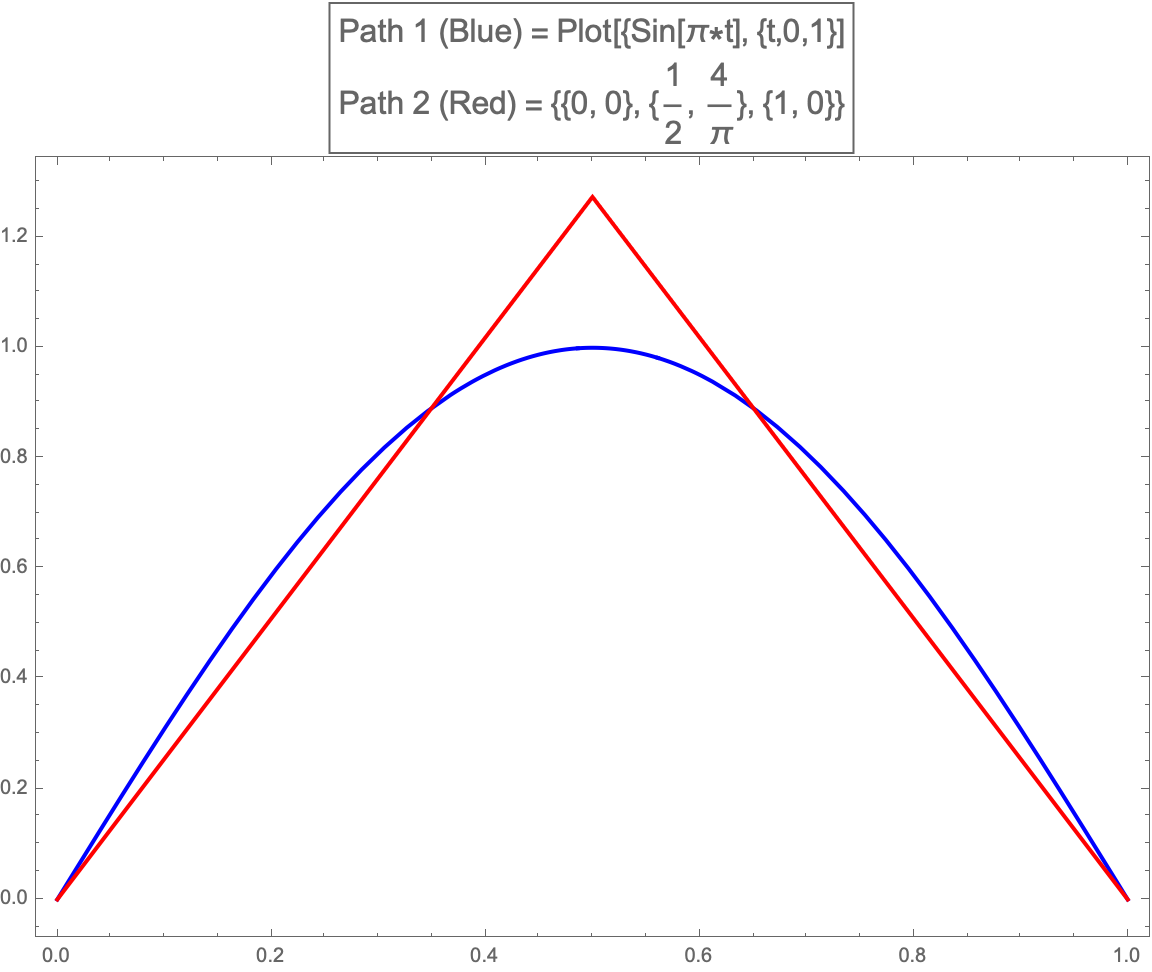
\includegraphics[scale=0.5]{figures/FitSint1l2}\hfill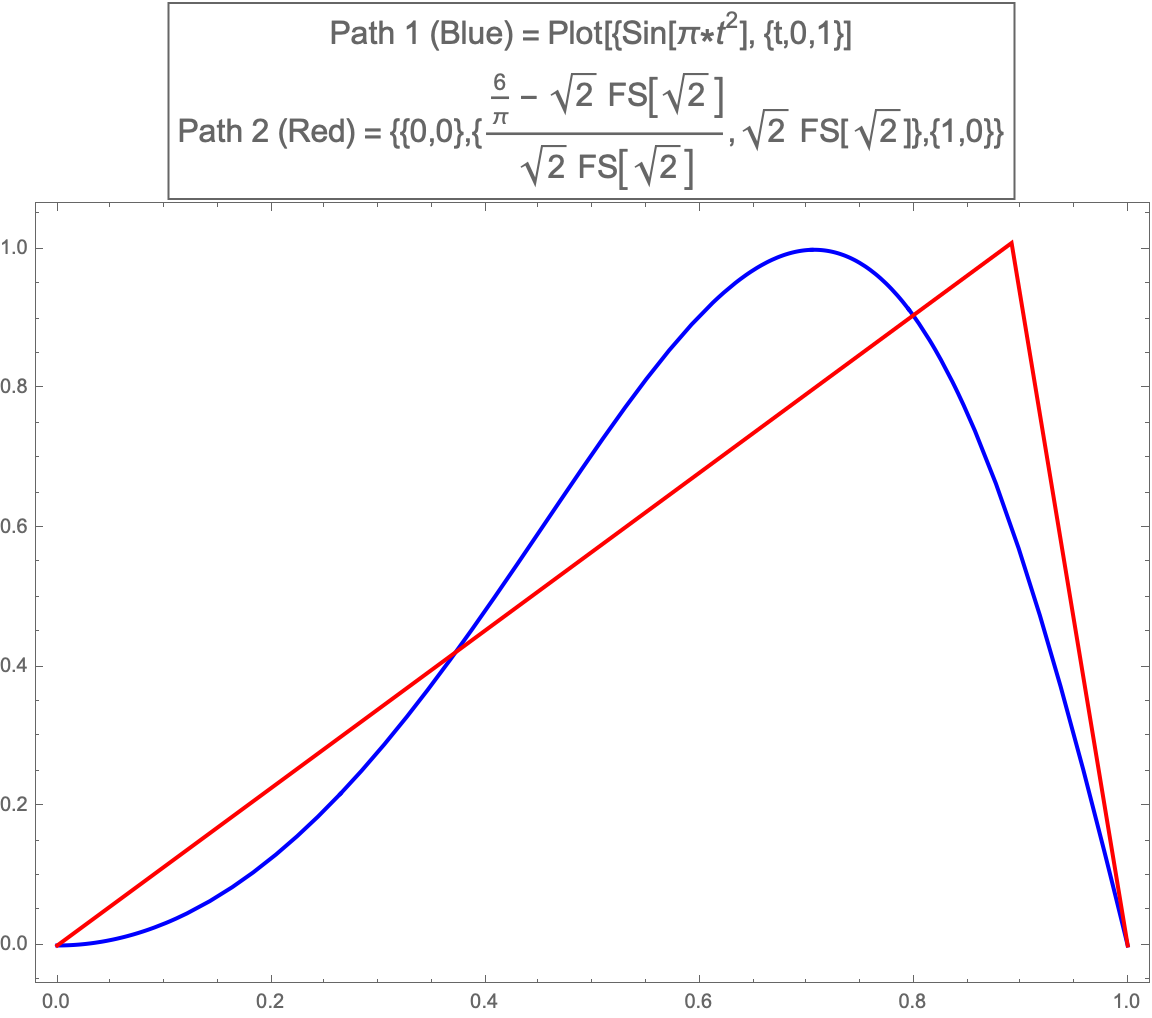
\includegraphics[scale=0.5]{figures/FitSint2l2}
\caption{Two-segment fits to $\{t,\sin(\pi t)\}$ and $\{t,\sin(\pi t^{2})\}$.\label{fig:sint12l2}}
\end{figure}

\begin{figure}[H]
\centering
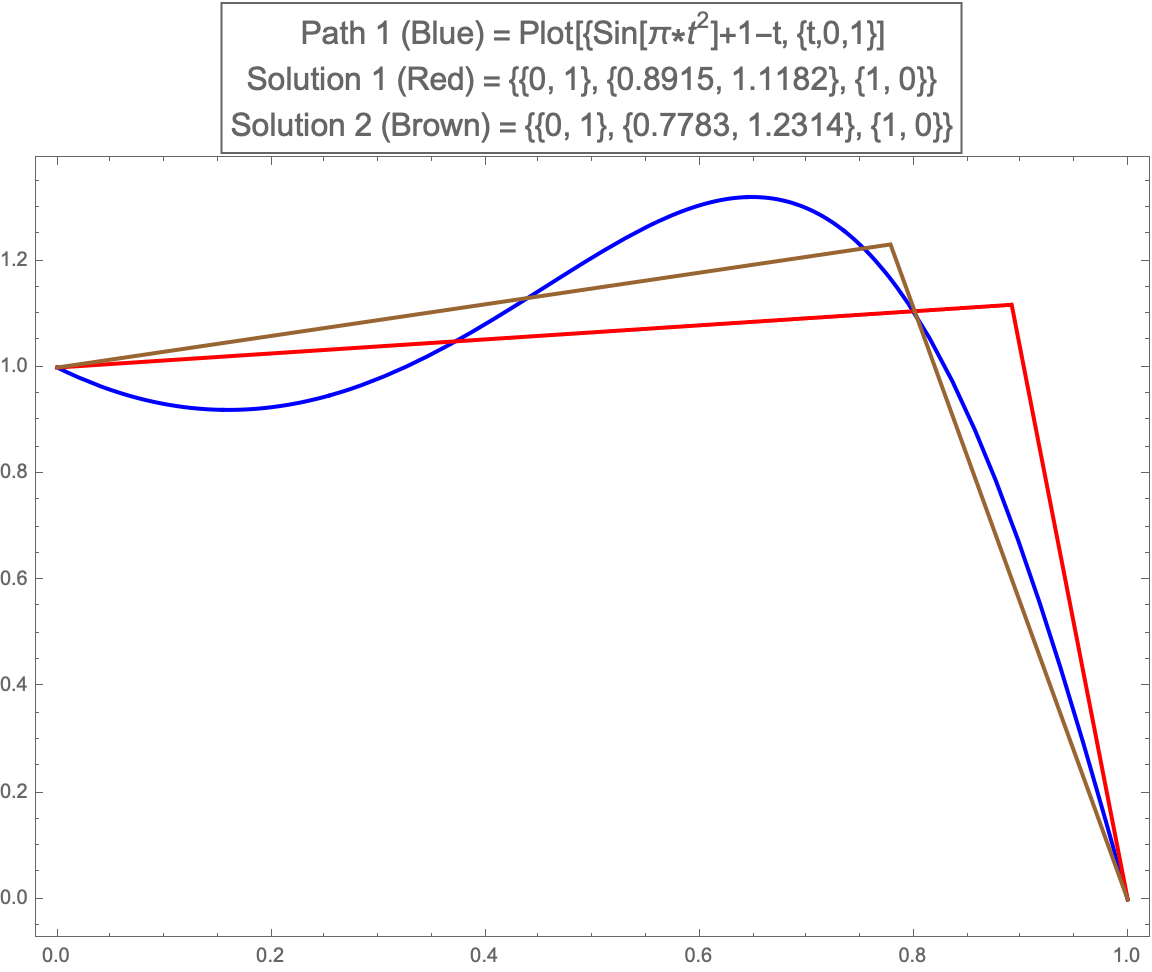
\includegraphics[scale=0.5]{figures/FitSint21tl2}
\caption{The two two-segment fits to $\{t,\sin(\pi t^{2})+1-t\}$.\label{fig:sint21tl2}}
\end{figure}

For an additive target $\{t,\alpha t^{a}+\beta t^{b}\}$ with $a,b>0$,
the core signature decomposes additively in $z_{1},z_{2},z_{1,2},z_{1,1,2}$
across the two summand paths and adds a single cross-term in $z_{1,2,2}$.
This explains why the choice of which equation to drop affects the
fit qualitatively: for paths well-modelled as a primary component
plus a linear drift, dropping equation $\#4$ recovers the primary
component more faithfully.

\subsection{Adversarial cases\label{subsec:Adversarial}}

The two-piece inversion fails when the closed forms of Appendix \ref{app:ChenSolutions}
have vanishing denominators. The two relevant degeneracies are:
\begin{itemize}
\item $z_{1}z_{2}-2z_{1,2}=0$ (Lévy area zero relative to the chord),
where the intermediate point's distance from the chord is undetermined;
\item $z_{2}=0$, which removes one of the two solutions.
\end{itemize}
Both situations occur for $\{t,\sin(2\pi t)\}$ and similar oscillatory
targets where one period of the oscillation cancels another. The
remedy is to use three or more pieces.

\subsection{Three pieces and beyond\label{subsec:More-pieces}}

Adding a third segment introduces three new unknowns and two more
core entries (level 4) into the system. The resulting equations are
listed in Appendix \ref{app:ChenSolutions}. For four or five segments
we move to level 5 of the signature; the choice of which equation
to drop in the resulting overdetermined system is no longer canonical,
and the non-linearity of the equations makes symbolic solution prohibitively
slow. We solve numerically through the regression of Section \ref{subsec:Inversion-as-regression}.

Figures \ref{fig:sinpaths4pts} and \ref{fig:sin2paths4pts} show four-
and five-segment fits to $\{t,\sin(k\pi t)\}$ and $\{t,\sin(k\pi t^{2})\}$
for $k=1,2,3$. The recovery is exact at the algebraic level for piecewise
linear targets and degrades gracefully for oscillatory smooth targets,
in line with the per-segment-frequency analysis of Section \ref{subsec:Inversion-as-regression}.

\begin{figure}[H]
\centering
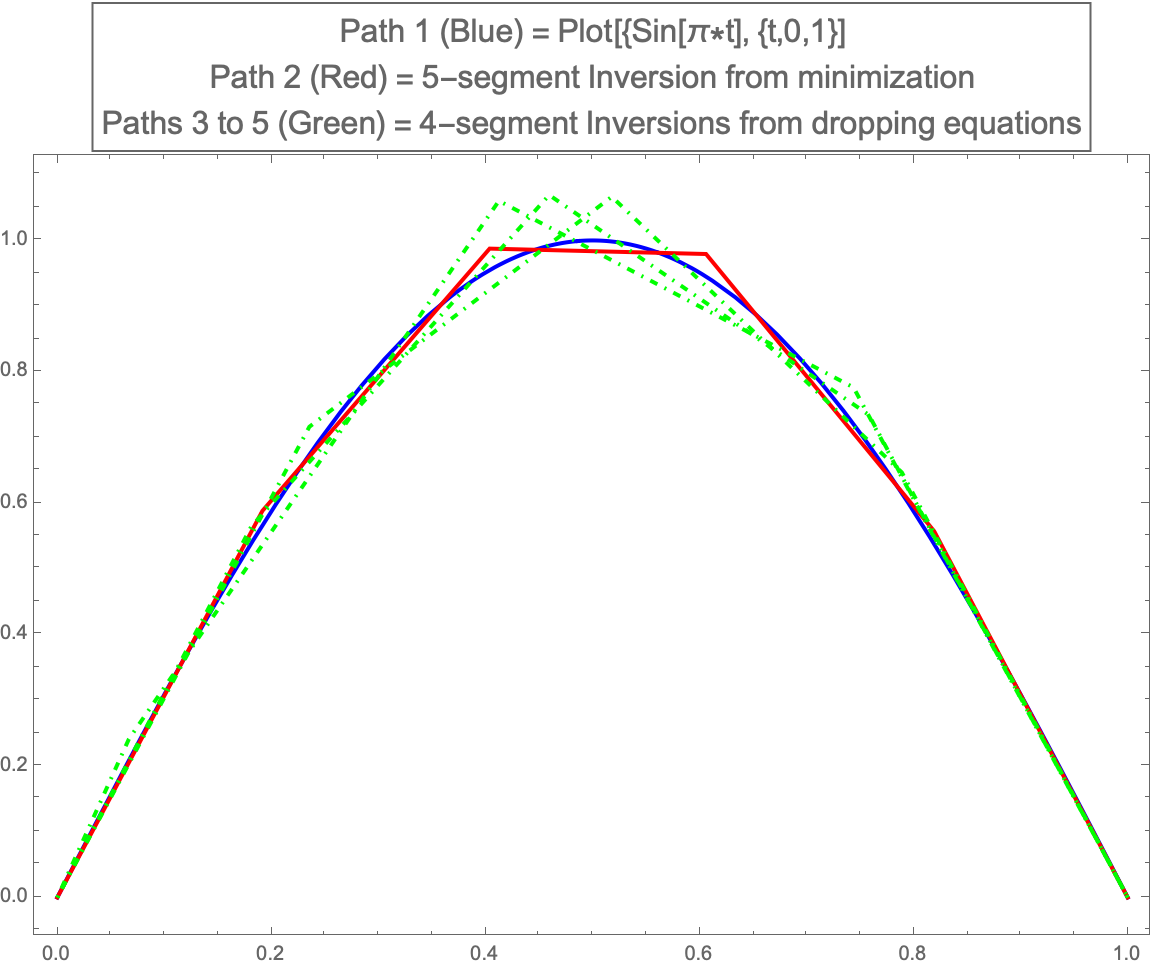
\includegraphics[scale=0.5]{figures/Fit4pPath1}\hfill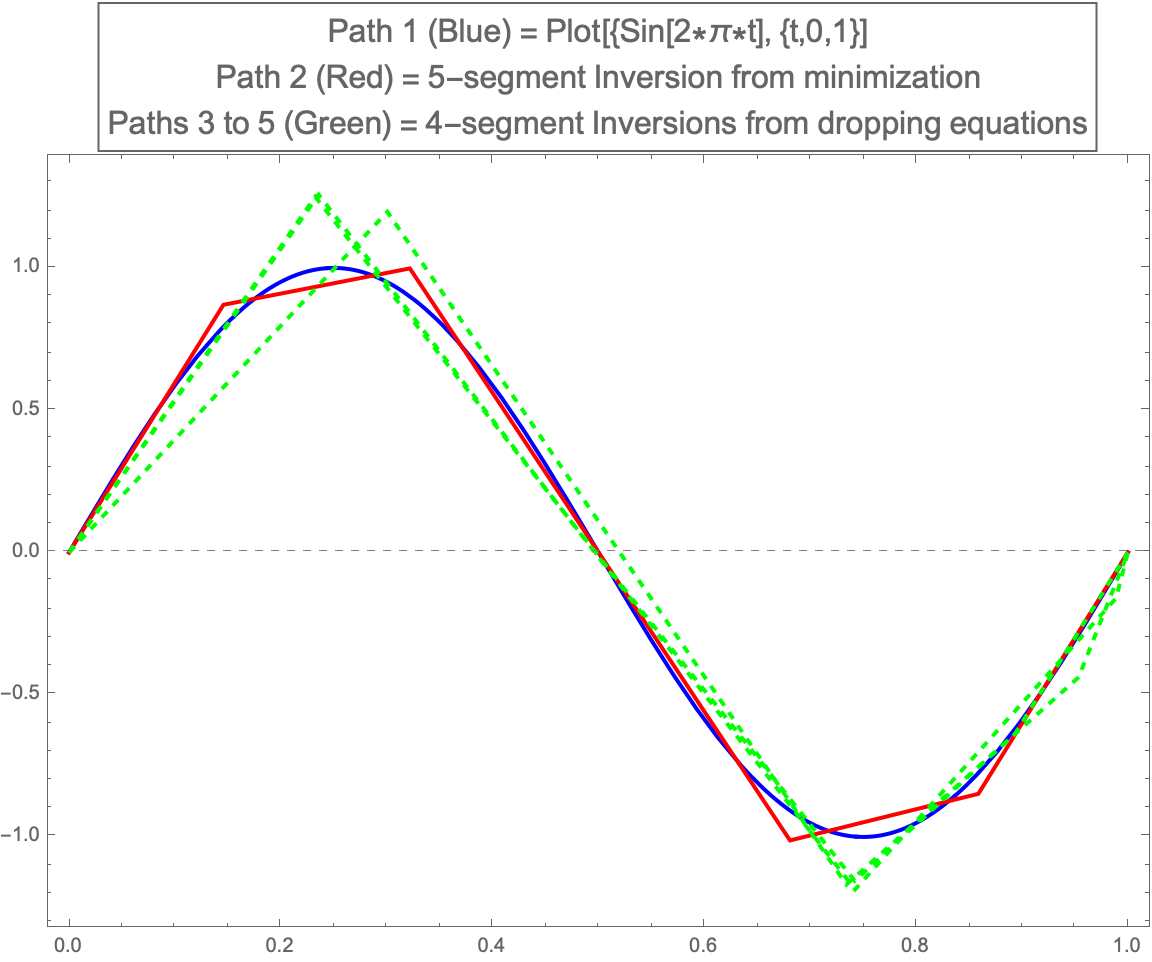
\includegraphics[scale=0.5]{figures/Fit4pPath2}
\caption{Fits of 4 and 5 segments to $\{t,\sin(k\pi t)\}$.\label{fig:sinpaths4pts}}
\end{figure}

\begin{figure}[H]
\centering
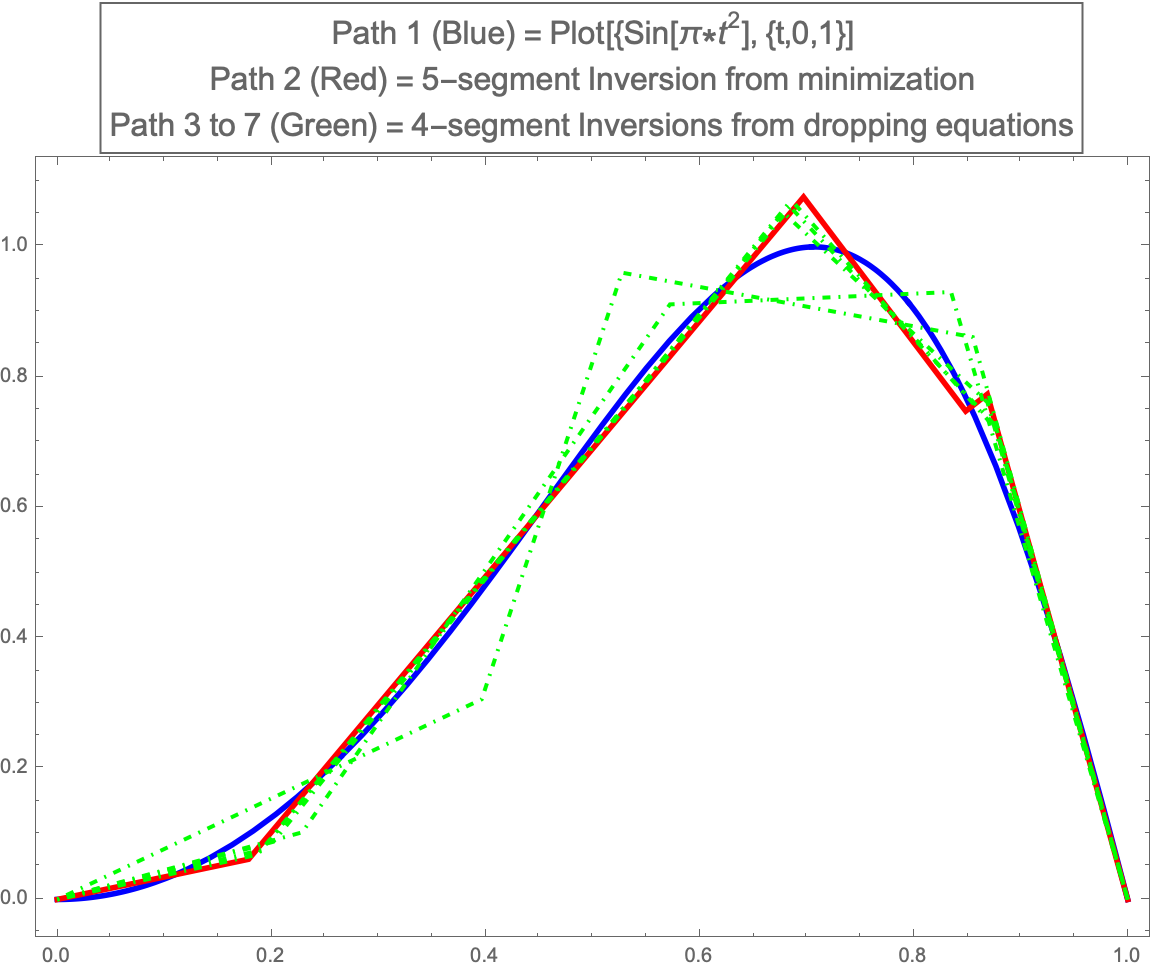
\includegraphics[scale=0.5]{figures/Fit4pPath3}\hfill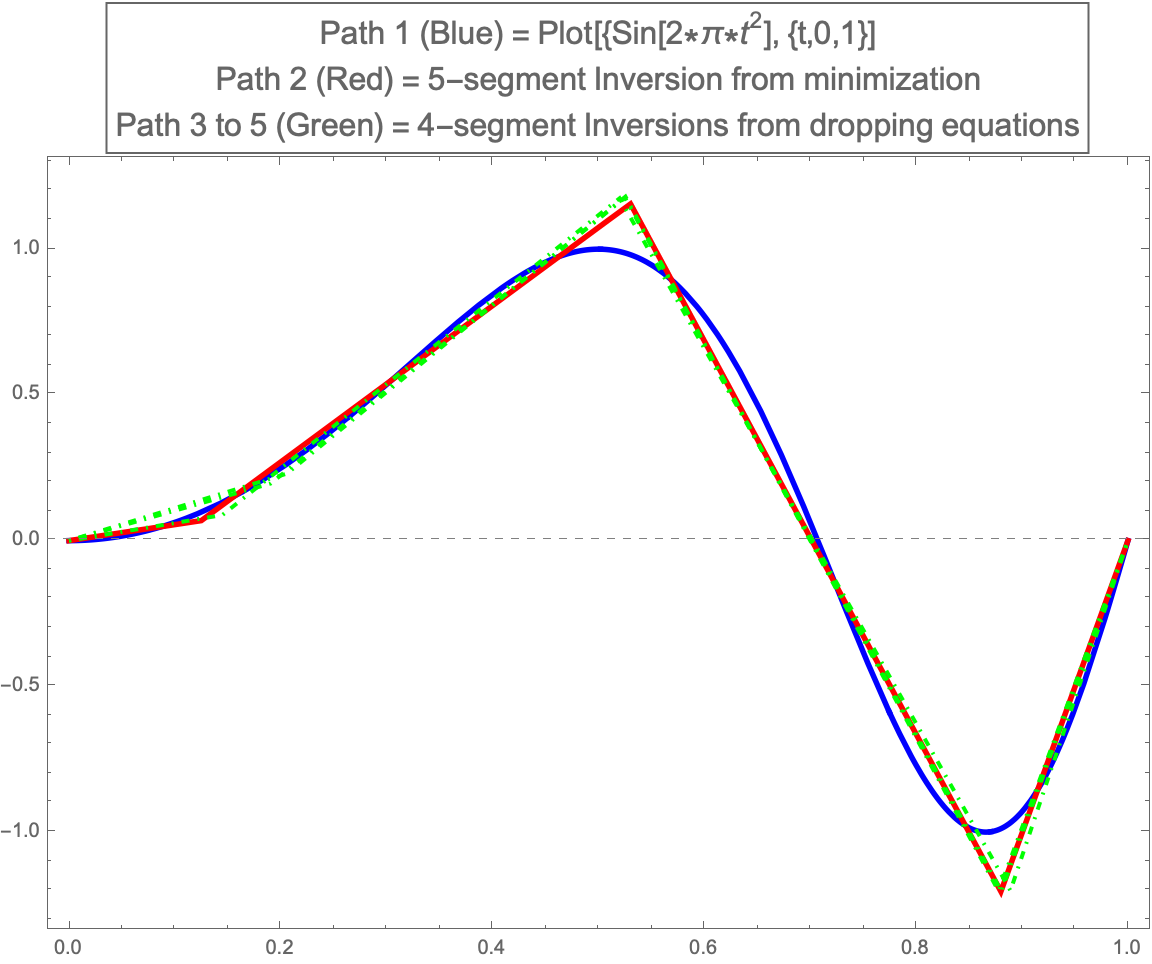
\includegraphics[scale=0.5]{figures/Fit4pPath4}
\caption{Fits of 4 and 5 segments to $\{t,\sin(k\pi t^{2})\}$.\label{fig:sin2paths4pts}}
\end{figure}

\subsection{General 2d paths\label{subsec:General-2d-paths}}

For a general path $X(t)=(f(t),g(t))$, both coordinates carry information
and the path may loop. We replace each segment by $\{a_{j}t,b_{j}t\}$
and apply the same Chen-based matching, filtering out reconstructed
paths whose total length exceeds an empirical threshold (chosen by
inspection of the algebraic-extraneous solutions in each test case).
\emph{This length-based filter is heuristic, not algebraic: it discards
solutions of the Chen system whose excess arclength signals a spurious
algebraic root rather than a geometric reconstruction. A principled
replacement --- e.g.\ a constraint derived from the path recovery
degree of \cite{splines} or from the regression of Section \ref{subsec:Inversion-as-regression}
--- is desirable and is left to future work.}

For the semicircle $\{\cos(\pi t),\sin(\pi t)\}$ with $t\in[0,1]$
the three-piece fit recovers the visual outline cleanly (Figure \ref{fig:semicircle}).
For the digit ``5'' described by the eight control points
\[
\bigl(\,0,\,20,\,64,\,79,\,35,\,37,\,71,\,100\,;\;0,\,-3,\,13,\,47,\,54,\,77,\,96,\,93\,\bigr)\,,
\]
both the three-piece and five-piece inversions reproduce the topology
of the digit (Figures \ref{fig:digit5_3} and \ref{fig:digit5_5});
the five-piece fit, computed via \texttt{NMinimize} with random search,
matches the original 7-segment piecewise linear path to visual accuracy.

\begin{figure}[H]
\centering
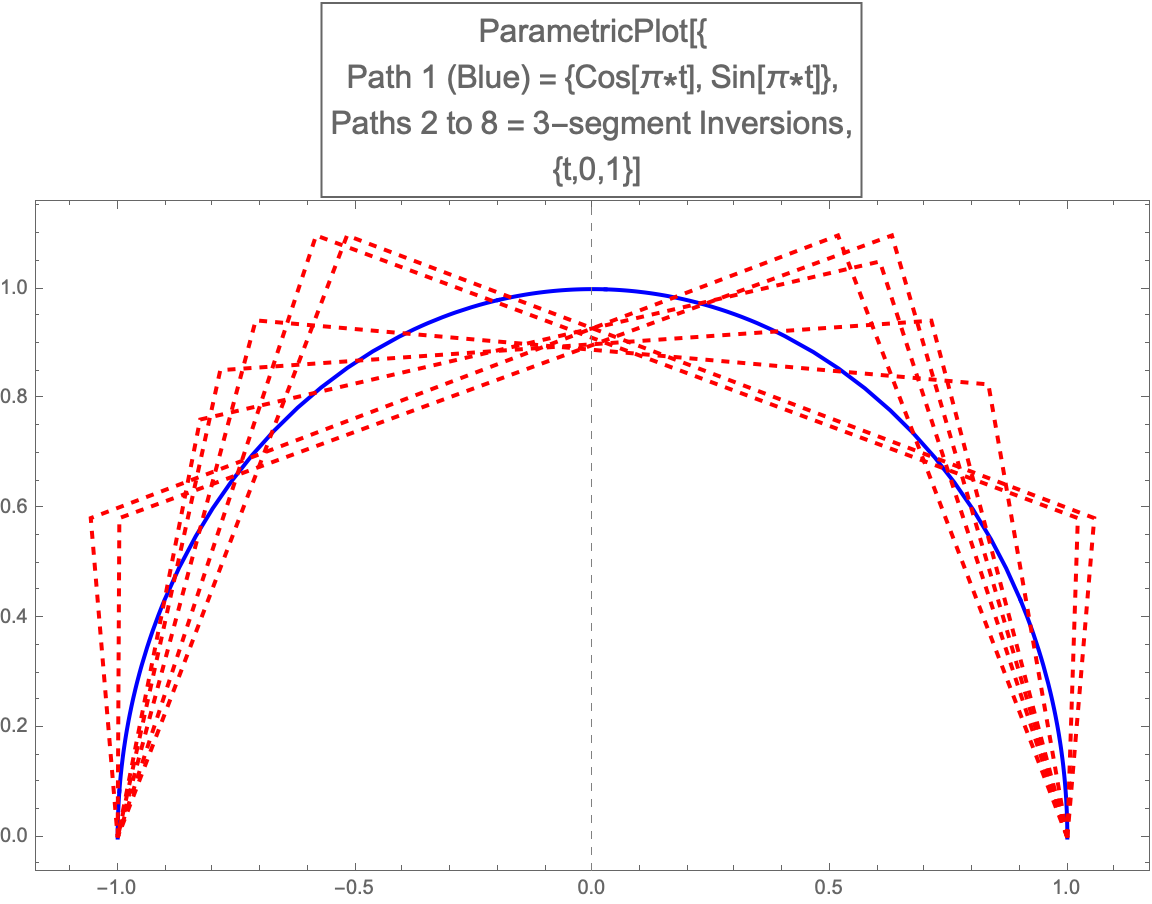
\includegraphics[scale=0.45]{figures/SemiCircle3}\hfill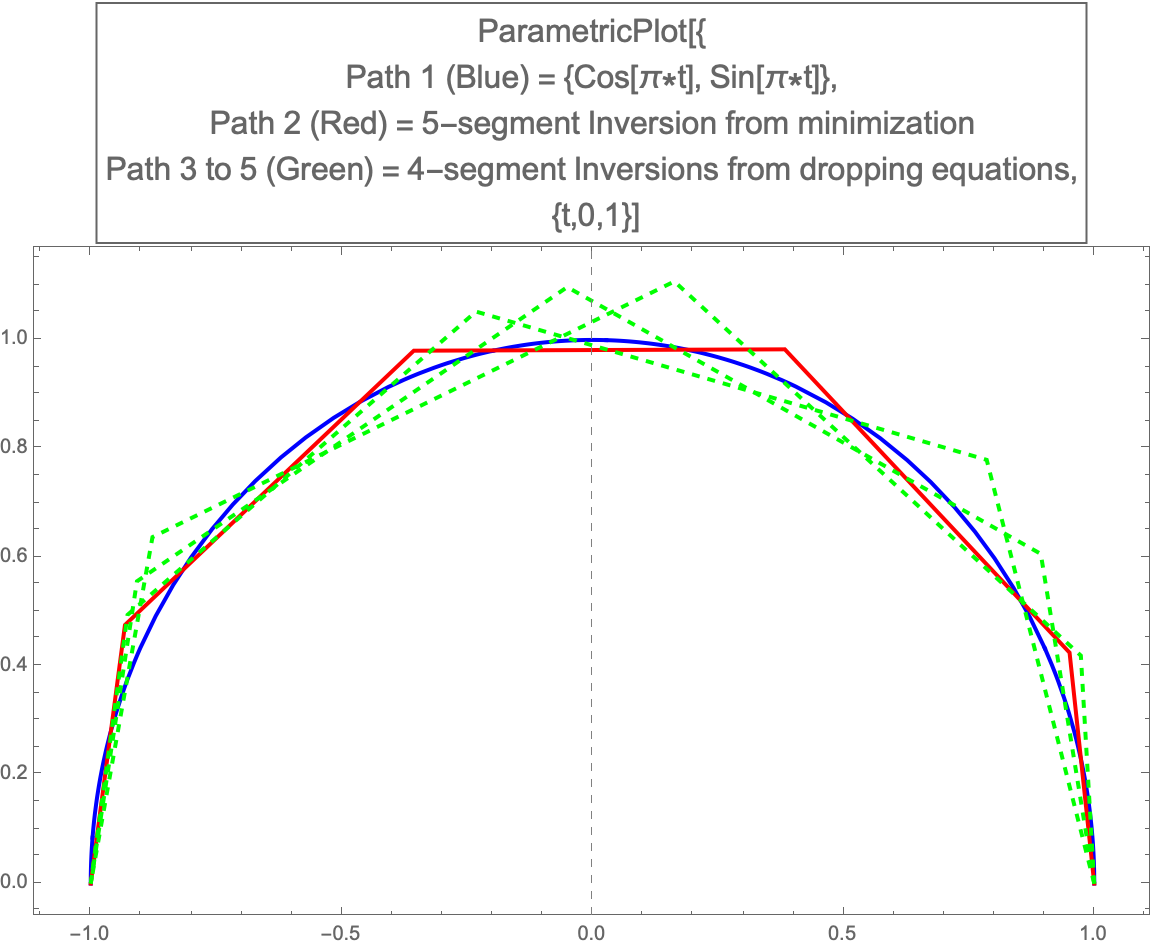
\includegraphics[scale=0.45]{figures/SemiCircle4}
\caption{Three- and four-piece inversions of the semicircle $\{\cos(\pi t),\sin(\pi t)\}$.\label{fig:semicircle}}
\end{figure}

\begin{figure}[H]
\centering
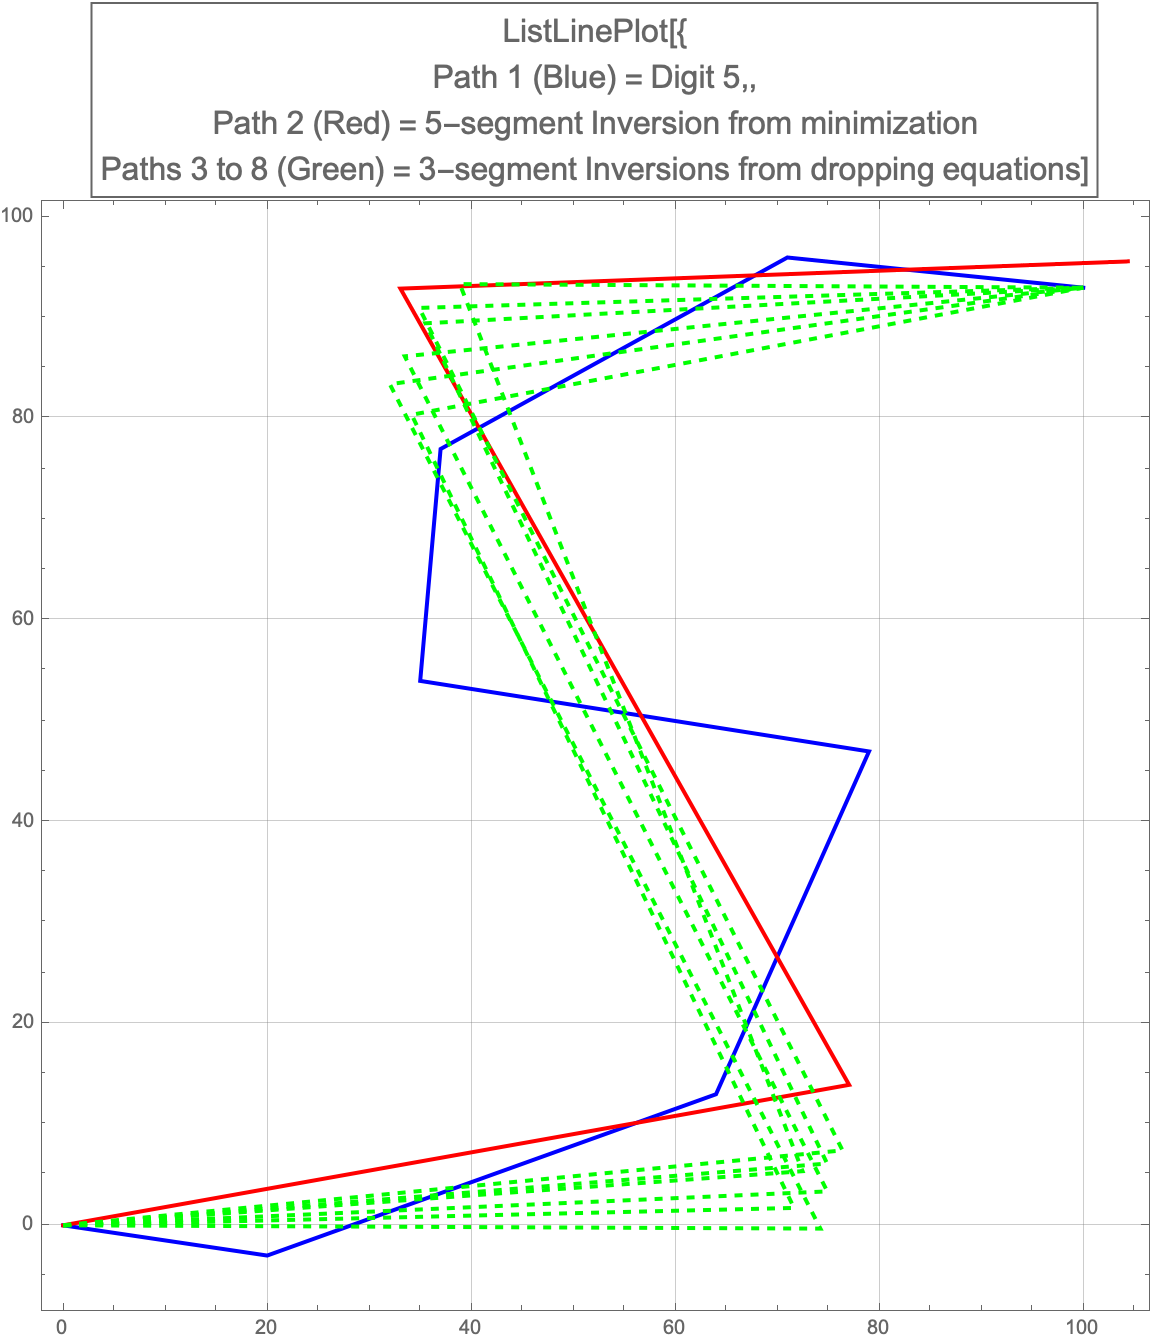
\includegraphics[scale=0.5]{figures/Digit5_3}
\caption{Three-segment inversion of the digit 5.\label{fig:digit5_3}}
\end{figure}

\begin{figure}[H]
\centering
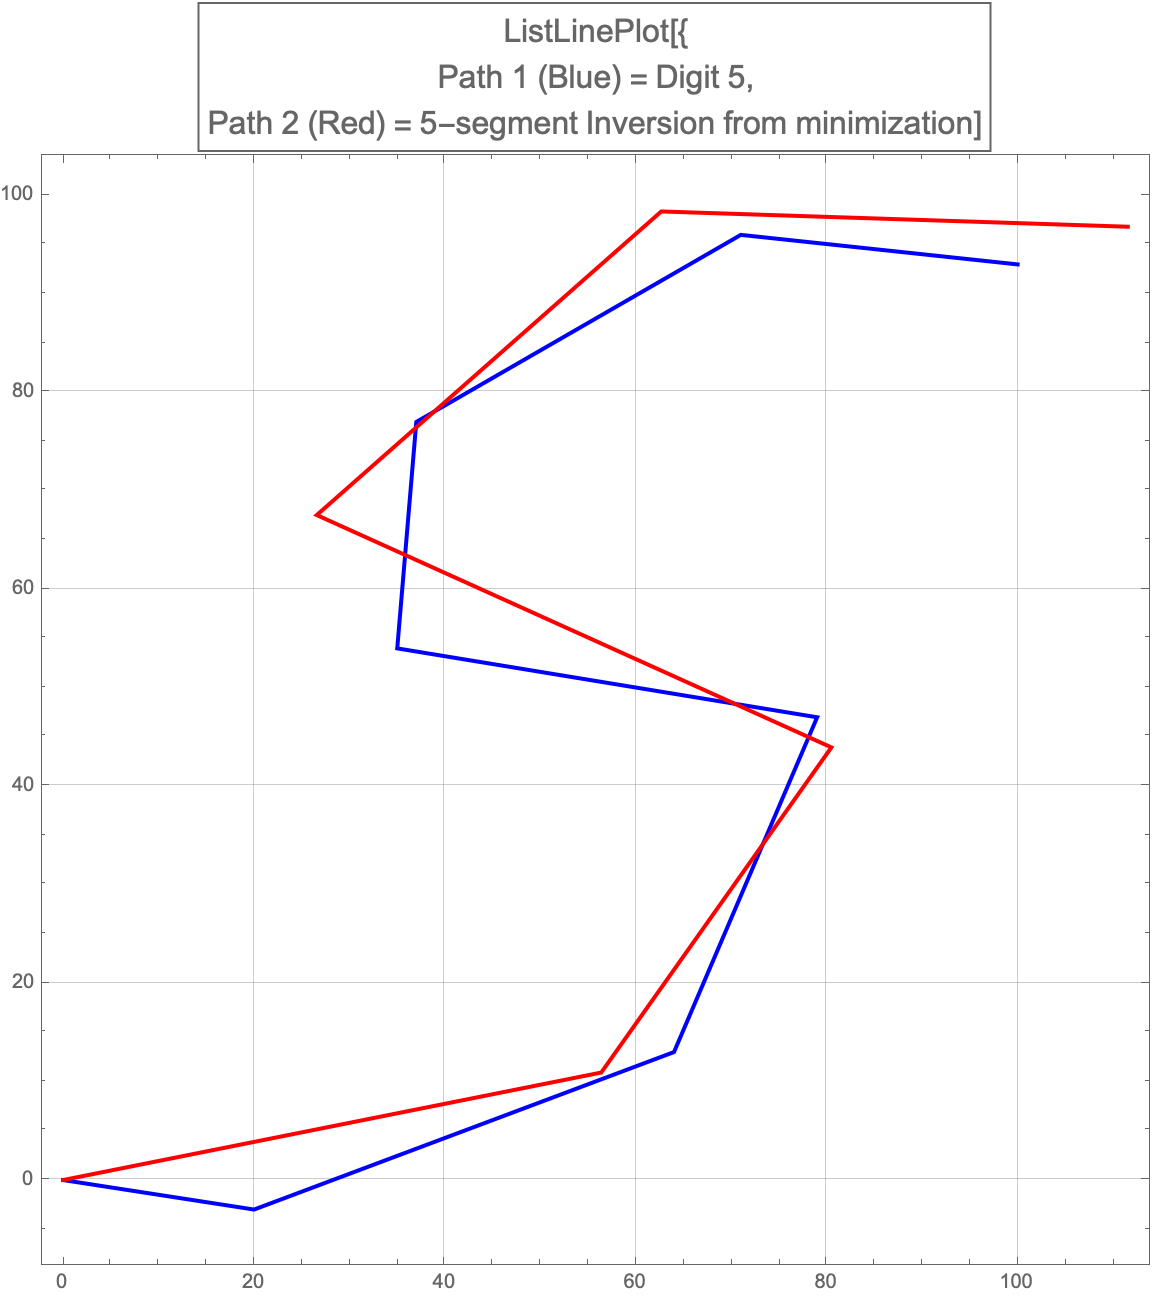
\includegraphics[scale=0.5]{figures/Digit5_5}
\caption{Five-segment inversion of the digit 5.\label{fig:digit5_5}}
\end{figure}

\subsection{Inversion as weighted regression in signature space\label{subsec:Inversion-as-regression}}

For piecewise linear paths with $n$ segments the inversion problem
has $2n-2$ free parameters once the endpoints are pinned, exactly
matching the number of independent core entries up to level $n$ from
Corollary \ref{cor:core-size}. To use signature information beyond
level $n$ --- which the per-segment-frequency analysis below shows
is necessary for oscillatory targets --- the system becomes overdetermined,
and we minimise a weighted least-squares objective in signature space:
\begin{equation}
\theta^{\star}\;=\;\underset{\theta}{\arg\min}\;\sum_{w\in\mathcal{L}_{m}}w_{w}\bigl(\sigma_{w}[g_{\theta}]-\sigma_{w}[X]\bigr)^{2}\,,\label{eq:weighted-regression}
\end{equation}
where $\mathcal{L}_{m}$ is the set of Lyndon words up to level $m$.
The companion notebook uses level-only weights $w_{w}=W_{|w|}$ with
$W_{\bullet}=\{50,50,30,10,10,3,3,3\}$ across the core indices and
\texttt{DifferentialEvolution} as the optimiser. For targets within
the parametric class $\mathcal{P}_{n}$ --- i.e.\ signatures generated
from a piecewise-linear path of the right segment count --- the regression
recovers the generating parameters to floating-point precision. For
smooth out-of-class targets, the regression converges to a weighted
least-squares optimum that differs from the closed-form algebraic
solutions of Appendix \ref{app:ChenSolutions} and achieves a strictly
lower $J(\theta^{\star})$ than any of them; the gap quantifies how
much cross-residual budget the regression is exploiting. The practical
implementation choices are summarised in Algorithm \ref{alg:inversion-regression}.

\begin{algorithm}[H]
\caption{Core-signature inversion via signature-space regression\label{alg:inversion-regression}}
\smallskip{}

\textbf{Inputs.} Target core signature $\{\sigma_{w}[X]:w\in\mathcal{L}_{m}\}$;
number of segments $n$; truncation level $m\geq n$; level-weight schedule
$W=(W_{1},\ldots,W_{m})$.

\textbf{Output.} Piecewise-linear path $g_{\theta^{\star}}\in\mathcal{P}_{n}$
whose core signature matches $\sigma[X]$ in the weighted-least-squares
sense of \eqref{eq:weighted-regression}.

\smallskip{}
\begin{enumerate}
\item \emph{Parametrise.} Write $g_{\theta}$ as a piecewise-linear path
with $n$ segments parametrised by $\theta=(\beta_{1},\ldots,\beta_{n};\,t_{1},\ldots,t_{n-1})$,
endpoints pinned, subject to the ordering constraint $0<t_{1}<\cdots<t_{n-1}<T$.

\item \emph{Compile the objective.} Compute the core signature $\sigma_{w}[g_{\theta}]$
symbolically using Chen's identity \eqref{eq:ChenIndex} and the line-segment
formula \eqref{eq:LineSignature}, for all $w\in\mathcal{L}_{m}$. This
step is one-time per $(n,m)$ pair and produces explicit polynomials
in $\theta$. Form $J(\theta)=\sum_{w\in\mathcal{L}_{m}}W_{|w|}\bigl(\sigma_{w}[g_{\theta}]-\sigma_{w}[X]\bigr)^{2}$.

\item \emph{Optimise.} Call \texttt{NMinimize[$J[\theta]$, constraints,
$\theta$, Method $\to$ DifferentialEvolution]}. Tolerances: \texttt{AccuracyGoal
$\to$ 8}, \texttt{PrecisionGoal $\to$ 8}, \texttt{MaxIterations $\to$
500}. The Mathematica defaults for \texttt{DifferentialEvolution}
(population size $\approx30\dim(\theta)$, \texttt{CrossProbability
$\to$ 0.5}, \texttt{ScalingFactor $\to$ 0.6}) suffice for $n\leq4$
segments and $m\leq6$ levels. Typical convergence on smooth out-of-class
targets at level $m=3$ truncation is to $J(\theta^{\star})$ of order
$10^{-3}$ and improves with $m$; on in-class targets the regression
reaches floating-point precision.

\item \emph{Diagnose and return.} Empirically, on the time-augmented
targets tested in this paper at $n=2$, DE converges to a single basin
across independent \texttt{RandomSeed} values, and the spread of $J(\theta^{\star})$
across seeds serves as a useful convergence diagnostic. At higher
segment counts the universal-variety path-recovery-degree formalism
of \cite{splines} (Definition~6.1; their Table~3 records $\mathrm{PRdeg}=4$
for piecewise linear paths with four segments at $d=2$, $k=4$) implies
that the regression objective may have multiple basins corresponding
to algebraically distinct paths with the same level-$m$ signature.
Whether the weighted regression \eqref{eq:weighted-regression} retains
a single dominant basin in such regimes is an open question; the cross-seed
$J(\theta^{\star})$ spread is the appropriate empirical diagnostic. The algebraic Solution-$\#1$ and Solution-$\#2$ of Appendix
\ref{app:ChenSolutions} are \emph{not} local minima of $J$: they
solve specific determined sub-systems (drop equation $\#4$ or $\#5$)
and have non-zero gradient with respect to the dropped equation's
residual. They are nevertheless useful as diagnostic anchors --- $J(\theta^{\star})$
should be bounded above by $\min_{k}J(\mathrm{Sol}\text{-}\#k)$, and
a small gap indicates a well-conditioned regression while a substantial
gap indicates the regression is exploiting the cross-residual budget
heavily. When the user wants the specific Solution-$\#k$ for downstream
reasons (smoothness, monotonicity, or a closed-form expression in
the target signature), they should solve the corresponding determined
sub-system of Appendix \ref{app:ChenSolutions} directly rather than
the regression. Return $\theta^{\star}$ and $g_{\theta^{\star}}$.
\end{enumerate}
\end{algorithm}

\begin{remark}[Comparison-baseline parameters]
The empirical-coincidence claim of Section \ref{subsubsec:L1-coincidence}
below uses the companion notebook \nbfile{Frechet.nb}, which runs
an independent $(\mu+\lambda)$-evolution strategy on the mean-$L^{1}$
objective rather than the signature-space objective \eqref{eq:weighted-regression}.
Parameters: population size $250$; Gaussian mutation with standard
deviation $\sigma=0.025$ on interior breakpoints; elite-plus-mutation
selection with fresh random ``islands'' injected each generation;
fixed $50$ generations with no early-stopping criterion. The mean-$L^{1}$
algorithm is independent of Algorithm \ref{alg:inversion-regression}
and serves to establish that the signature-space minimiser coincides
with the optimal $L^{1}$ piecewise-linear approximant on the same
partition class.
\end{remark}

\begin{remark}[Why the level scaling matters]
Signature entries at level $k$ on a path of duration $T$ scale as
$O(T^{k}/k!)$ via the simplex of integration. Without compensating
weights the objective is dominated by noise in the high-level entries
and loses sensitivity to the dominant low-level structure. The empirical
weights above are decreasing with level but slower than $1/k!$; an
explicit theoretical choice $w_{w}\propto(k!)^{2}/T^{2k}$ would normalise
residuals to comparable magnitudes across levels, and is the form
suggested by the asymptotic analysis below.
\end{remark}

\subsubsection{Signature entries as iterated path moments}

For $X(t)=(t,f(t))$ on $[0,T]$, integration by parts gives
\begin{align}
\sigma_{1,2}[X] & =Tf(T)-\textstyle\int_{0}^{T}f(t)\,dt\,,\label{eq:moment-12}\\
\sigma_{1,1,2}[X] & =\textstyle\frac{T^{2}}{2}f(T)-\int_{0}^{T}t\,f(t)\,dt\,,
\end{align}
and so on. Every Lyndon-word signature entry of a time-augmented path
is a polynomial in the moments $M_{k}(f)=\int_{0}^{T}t^{k}f(t)\,dt$
and the boundary values of $f$. To leading order in the level grading,
the regression \eqref{eq:weighted-regression} is therefore a weighted
moment-matching problem,
\begin{equation}
J(\theta)\;\simeq\;\sum_{k=0}^{m-1}\widetilde{w}_{k}\bigl(M_{k}(g_{\theta})-M_{k}(f)\bigr)^{2}\,,\label{eq:moment-regression}
\end{equation}
with effective weights $\widetilde{w}_{k}$ derived from the $w_{w}$
through the integration-by-parts identities. By the classical Hausdorff
moment problem and its quantitative refinements (\cite{Talenti}),
matching the first $m$ moments of $f\in C^{s}([0,T])$ pins down
$f$ in $L^{1}$ to order $O(m^{-s})$.

\subsubsection{Empirical coincidence with mean $L^{1}$ minimisation\label{subsubsec:L1-coincidence}}

The companion notebook \nbfile{Frechet.nb} runs an evolutionary algorithm
on the four-segment class minimising the mean pointwise distance
\[
\mathrm{meandist}(g_{\theta},f)\;=\;\tfrac{1}{N+1}\sum_{i=0}^{N}\bigl|f(t_{i})-g_{\theta}(t_{i})\bigr|\,,\qquad t_{i}=iT/N\,.
\]
On the target $f(t)=\sin(2\pi t^{2})$ with $T=1$ and $N=1000$, the
algorithm converges robustly across independent seeds to a piecewise-linear
approximation whose interior breakpoints agree to within a few percent
with those found by the algebraic core-signature inversion, but \emph{not}
to a common optimum: the two algorithms minimise structurally different
objectives --- signature-space residual sum for the algebraic inversion,
mean $L^{1}$ distance for the evolutionary algorithm --- and converge
to distinct nearby minima rather than to a shared root. Numerical verification
(Python port of both algorithms, population $250$ over $200$ generations
across $10$ independent seeds against a multi-start algebraic Chen solver)
recovers the algebraic root at machine precision and the mean-$L^{1}$
optimum at a $\sim11\%$ lower mean-$L^{1}$ value than the algebraic
root, confirming the two minima are genuinely distinct. This is the
multi-segment analogue of the single-segment $4.7\%$ obstruction noted
in Remark \ref{rem:single-segment-obstruction} below.

\begin{remark}[On the name ``Fréchet'']
Because the two paths share the time coordinate, $\mathrm{EuclideanDistance}((t,f),(t,g_{\theta}))=|f-g_{\theta}|$,
so the notebook objective is mean $L^{1}$, not the Fréchet distance
between curves. The relevant comparison is therefore between the signature-regression
solution and the optimal piecewise-linear $L^{1}$ approximant on
the same partition class.
\end{remark}

A heuristic explanation for the coincidence is now visible from \eqref{eq:moment-regression}:
both methods determine the breakpoints by first-order conditions on
identical leading moments of $f$, differing only by terms of order
$\sup|f''|\cdot(\Delta t)^{2}$. We emphasise that this is an
approximation-theoretic intuition rather than a proof of identity
or norm equivalence; the conjectural status of the link is the
subject of Conjecture \ref{conj:norm-equivalence} below.

\subsubsection{The norm-equivalence conjecture}

\begin{conjecture}[Signature-norm equivalence]
\label{conj:norm-equivalence} Let $\mathcal{F}\subseteq C^{1}([0,T];\mathbb{R})$
be a class of paths of bounded derivative and $X=(t,f)$, $G=(t,g)$
for $f,g\in\mathcal{F}$. There exist weights $\{w_{w}\}_{w\in\mathcal{L}}$
depending only on $|w|$ and $T$, with $w_{w}\sim(k!)^{2}/T^{2k}$
for $|w|=k$, and a Sobolev exponent $s\geq0$ such that
\begin{equation}
\sum_{w\in\mathcal{L}}w_{w}\bigl(\sigma_{w}[G]-\sigma_{w}[X]\bigr)^{2}\;\asymp\;\|f-g\|_{H^{s}([0,T])}^{2}\label{eq:norm-equivalence}
\end{equation}
uniformly for $f,g$ in compact subsets of $\mathcal{F}$, with constants
of equivalence depending only on the diameter of the compact set in
$H^{s}$.
\end{conjecture}

\begin{remark}[Status]
We have: (i) the empirical coincidence on a finite test set; (ii)
the moment-matching reason of \eqref{eq:moment-regression}; (iii)
the classical link between moment matching and $L^{1}/L^{2}$ approximation.
We do not have: an explicit identification of $s$, the constants
of equivalence, or a proof for any subclass of $\mathcal{F}$ richer
than polynomials. The natural first-proof target is therefore the
class of \emph{polynomial paths} on $[0,T]$: the universal-variety
coordinates restricted to polynomial paths are described explicitly
in \cite{varieties} Section 5 and in \cite{learning}, and the moment-matching
identities of \eqref{eq:moment-12} reduce there to finite-dimensional
linear systems in the polynomial coefficients, so a proof of \eqref{eq:norm-equivalence}
at that level would not require new functional-analytic machinery.
A positive answer would identify the inversion of this section as
a Galerkin projection of $f$ onto $\mathcal{P}_{n}$ in a Sobolev
norm, with the level $m$ playing the role of the truncation parameter.

An empirical complement to a proof is to calibrate the weights $w_{w}$
on representative training sets --- by genetic search, gradient descent
through the inner least-squares, or otherwise --- and to test whether
the calibrated asymptotic matches the $(k!)^{2}/T^{2k}$ worst-case
form (expected for rough paths where level-$k$ entries can saturate
the $O(T^{k}/k!)$ bound and one wants each level to contribute comparably
to the objective), the empirically observed decreasing form (expected
for smooth targets where the actual entries shrink faster than the
worst-case bound, so signal-to-noise decreases with level and the
high-level weights should be small), or something between. Training
across \emph{both} smoothness regimes --- e.g., rough paths constructed
from fractional Brownian motion alongside smooth analytic targets ---
would identify the class on which the conjecture holds in the simple
$(k!)^{2}/T^{2k}$ form, the class on which the empirical decreasing
form is correct, and the cross-over between them. A target-dependent
weight scheme (e.g.\ a small map from target-signature features to
weights, learned end-to-end) is the natural construction if the cross-over
turns out to be smooth.
\end{remark}

\begin{remark}[Single-segment obstruction]
\label{rem:single-segment-obstruction}
A direct computation on the simplest case --- one free interior breakpoint
$(\tau,y)$ on $[0,T]$ with pinned endpoints --- shows that exact
matching of $\sigma_{1,2}$ alone fixes $y=(2/T)\int_{0}^{T}f$ independently
of $\tau$, while $L^{2}$-optimality fixes $y$ to a hat-function
inner product depending on $\tau$. For $f(t)=\sin(\pi t)$, $T=1$,
symmetry forces $\tau^{\star}=1/2$ and the values are $y_{\sigma}=4/\pi\approx1.273$
versus $y_{L^{2}}=12/\pi^{2}\approx1.216$, a 4.7\% discrepancy. The
conjecture is therefore not pointwise identity of the two minimisers
but norm equivalence in the overdetermined regime.
\end{remark}

\subsubsection{Concatenation and the frequency-to-level correspondence}

By Chen \eqref{eq:ChenIdentity} and the linearity of moments, segment-wise
regression errors compose into a global error bounded by their sum:
for partitions $\{0=\tau_{0}<\cdots<\tau_{N}=T\}$ and per-segment
approximations $g^{(i)}$,
\begin{equation}
\sum_{w\in\mathcal{L}_{m}}w_{w}\bigl(\sigma_{w}[g]-\sigma_{w}[X]\bigr)^{2}\;\leq\;C(m,N)\,\sum_{i=1}^{N}\sum_{w\in\mathcal{L}_{m}}w_{w}\bigl(\sigma_{w}[g^{(i)}]-\sigma_{w}[X^{(i)}]\bigr)^{2}\,,\label{eq:concatenation-bound}
\end{equation}
with $C(m,N)$ polynomial in $N$ and exponential in $m$ from the
binomial expansions in \eqref{eq:ChenIndex}. This is the structural
reason why the segment-by-segment inversion of Section \ref{subsec:More-pieces}
is consistent with a global signature regression: per-segment errors
add additively, and a target $f$ of characteristic frequency $\omega_{0}$
needs $N\sim\omega_{0}T$ segments of length $\Delta t\sim1/\omega_{0}$
to keep the per-segment level requirement bounded. The global $L^{1}$
error then scales as $O(N^{-(m+1)})$ for $f\in C^{m+1}$, matching
classical piecewise-polynomial approximation rates.

%% =========================================================================
\section{Conclusions and forthcoming work}
%% =========================================================================

We introduced core signatures, identified them structurally with the
Lyndon coordinates of the universal step-$n$ free nilpotent Lie group
$G^{n}(\mathbb{R}^{d})$ (Proposition \ref{prop:lyndon-transcendence}
plus Corollary \ref{prop:core-is-lyndon}),
sized them via Witt's formula (Corollary \ref{cor:core-size}), and
gave a constructive Gröbner-basis algorithm for expressing any signature
entry in terms of the core. We then used Chen's identity to invert
core signatures into piecewise linear paths of two, three, or more
segments, and reframed the multi-segment case as a weighted nonlinear
least-squares regression in signature space whose minimiser empirically
coincides with the optimal piecewise-linear $L^{1}$ approximant.
Conjecture \ref{conj:norm-equivalence} states the norm-equivalence
result that would make this coincidence rigorous; the moment-matching
intuition of Section \ref{subsec:Inversion-as-regression} and the
single-segment computation give partial support and identify the precise
form a proof would need to take.

The application of the core-signature framework to interest-rate term
structures and other financial term-structure objects is the subject
of a forthcoming paper, in which we apply the inversion to the historical
USD Treasury and Brazilian DI futures curves to extract a low-dimensional
geometric encoding of the curve dynamics. Two analytical questions
left open here are (i) the explicit identification of the Sobolev
exponent $s$ and the constants of equivalence in \eqref{eq:norm-equivalence},
and (ii) the vector-valued generalisation of the moment-matching dictionary
required for the term-structure setting where path components are
correlated.

The core-signature framework has also been picked up in practitioner
work on quantitative-trading futuretesting; see \cite{bloch_futuretesting}.

We thank Sam Cohen (Oxford) for helpful discussions.

\paragraph{Use of AI assistance.}
The author used Anthropic's Claude to review the mathematical content
of the 2023 version of this paper, tighten the exposition, supply
the theoretical citation chain through the Lyndon basis theorem,
Poincaré--Birkhoff--Witt and Radford's theorem that identifies the
core variables with the Lyndon coordinates of $G^{n}(\mathbb{R}^{d})$,
and help draft the regression and norm-equivalence framing of Section
\ref{subsec:Inversion-as-regression}. All mathematical claims, the
choice of which results to state as conjectures, and the final form
of the paper are the author's responsibility.

\pagebreak{}

\begin{thebibliography}{Pfeffer, Seigal and Sturmfels (2018)}

\bibitem[Amendola, Friz and Sturmfels (2019)]{varieties}Amendola, C.,
Friz, P. and Sturmfels, B. (2019), ``Varieties of Signature Tensors'',
\href{https://arxiv.org/abs/1804.08325v3}{arXiv:1804.08325v3}

\bibitem[Amendola et al.\ (2025)]{macaulay2}Amendola, C., El Saliby, A.,
Lotter, F. and Reig Fité, O.\ (2025), ``Computing Path Signature Varieties
in Macaulay2'',
\href{https://arxiv.org/abs/2506.01429v1}{arXiv:2506.01429v1}

\bibitem[Amendola, Lotter and Schmitz (2026)]{splines}Amendola, C.,
Lotter, F. and Schmitz, L.\ (2026), ``Signature Varieties of Splines'',
\href{https://arxiv.org/abs/2602.13011v1}{arXiv:2602.13011v1}

\bibitem[Amendola and Schmitz (2025)]{barycenters}Amendola, C. and
Schmitz, L.\ (2025), ``Learning Barycenters from Signature Matrices'',
\href{https://arxiv.org/abs/2509.07815v1}{arXiv:2509.07815v1}

\bibitem[Bloch (2024)]{bloch_futuretesting}Bloch, D.\ (2024),
``Futuretesting Quantitative Strategies'', Working Paper, Quant
Finance Ltd, version 1.0.3 (revised 30 March 2024),
\href{https://papers.ssrn.com/sol3/papers.cfm?abstract_id=4647103}{SSRN:4647103}.

\bibitem[Chevyrev and Kormilitzin (2016)]{Primer}Chevyrev, I. and Kormilitzin, A.
(2016), ``A Primer on the Signature Method in Machine Learning'',
\href{https://arxiv.org/abs/1603.03788}{arXiv:1603.03788}

\bibitem[Fermanian (2021a)]{Fermanian_Thesis}Fermanian, A. (2021a),
``Learning time-dependent data with the signature transform'',
\href{https://theses.hal.science/tel-03507274}{PhD Thesis, Sorbonne Université LSPM}

\bibitem[Fermanian (2021b)]{embedding}Fermanian, A. (2021b),
``Embedding and learning with signatures'', Computational Statistics
\& Data Analysis 157, 107148,
\href{https://doi.org/10.1016/j.csda.2020.107148}{https://doi.org/10.1016/j.csda.2020.107148}

\bibitem[Fermanian et al.\ (2023)]{inversion}Fermanian, A., Chang, J.,
Lyons, T., and Biau, G. (2023), ``The insertion method to invert the
signature of a path'', \href{https://arxiv.org/abs/2304.01862v2}{arXiv:2304.01862v2}

\bibitem[Lyons, Caruana and Lévy (2007)]{Lyons}Lyons, T.~J., Caruana, M.,
and Lévy, T.\ (2007), \emph{Differential equations driven by rough paths},
volume 1908 of Lecture Notes in Mathematics, Springer, Berlin.

\bibitem[Pfeffer, Seigal and Sturmfels (2018)]{learning}Pfeffer, M.,
Seigal, A. and Sturmfels, B.\ (2018), ``Learning Paths from Signature
Tensors'', \href{https://arxiv.org/abs/1809.01588v2}{arXiv:1809.01588v2}

\bibitem[Reizenstein (2015)]{log signatures}Reizenstein, J.\ (2015),
``Calculation of Iterated-Integral Signatures and Log Signatures'',
\href{https://arxiv.org/abs/1712.02757v1}{arXiv:1712.02757v1}

\bibitem[Reizenstein (2016)]{iisignature CRISM}Reizenstein, J.\ (2016),
``Calculation of signatures'', CRISM workshop:\ Statistics for
Differential Equations Driven by Rough Paths.

\bibitem[Reizenstein (2018)]{iisignature}Reizenstein, J.\ (2018),
``The iisignature library'',
\href{https://arxiv.org/abs/1802.08252v1}{arXiv:1802.08252v1}

\bibitem[Reizenstein and Graham (2020)]{iisignature 1004}Reizenstein, J.
and Graham, B.\ (2020), ``Algorithm 1004: The Iisignature Library'',
ACM Trans.\ Math.\ Softw.\ 46, 1, Article 8,
\href{https://doi.org/10.1145/3371237}{https://doi.org/10.1145/3371237}

\bibitem[Riffo and Schmitz (2026)]{signaturetensorsjl}Riffo, G.\ and
Schmitz, L.\ (2026), ``SignatureTensors.jl: A Package for Signature
Tensors in Julia'',
\href{https://arxiv.org/abs/2604.19227v1}{arXiv:2604.19227v1}

\bibitem[Reutenauer (1993)]{Reutenauer}Reutenauer, C.\ (1993),
\emph{Free Lie Algebras}, London Mathematical Society Monographs,
New Series 7, Oxford Science Publications.

\bibitem[Schmitz (2025)]{tensorlearning}Schmitz, L.\ (2025), ``An
Efficient Algorithm for Tensor Learning'',
\href{https://arxiv.org/abs/2512.14218v1}{arXiv:2512.14218v1}

\bibitem[Talenti (1987)]{Talenti}Talenti, G.\ (1987), ``Recovering
a function from a finite number of moments'', Inverse Problems 3,
501--517,
\href{https://doi.org/10.1088/0266-5611/3/3/016}{https://doi.org/10.1088/0266-5611/3/3/016}

\end{thebibliography}

\pagebreak{}

\appendix
\part*{Appendix}

%% =========================================================================
\section{Substitution rules $Q_{m}$ for $d=2$\label{app:Q5}}
%% =========================================================================

The substitution rules below express every non-core signature entry
of $V_{1}\cup\cdots\cup V_{m}$ as a polynomial in $C_{m}$. The choice
of representative within each shuffle orbit is the lex-minimal one
(equivalently, the Lyndon representative of each primitive necklace).
$Q_{6}$ for $d\in\{2,3\}$ is exported in the companion notebook
\nbfile{CoreSignatures202412.nb}.

The cores referenced below are
\[
C_{1}=\{s_{1},s_{2}\}\,,\quad C_{2}=C_{1}\cup\{s_{1,2}\}\,,\quad C_{3}=C_{2}\cup\{s_{1,1,2},s_{1,2,2}\}\,,
\]
\[
C_{4}=C_{3}\cup\{s_{1,1,1,2},s_{1,1,2,2},s_{1,2,2,2}\}\,,
\]
\[
C_{5}=C_{4}\cup\{s_{1,1,1,1,2},s_{1,1,1,2,2},s_{1,1,2,1,2},s_{1,1,2,2,2},s_{1,2,1,2,2},s_{1,2,2,2,2}\}\,.
\]

\subsection{Level 2}
\begin{tabular}{|l|l|}
\hline
$s_{1,1}$ & $\frac{1}{2}s_{1}^{2}$\tabularnewline\hline
$s_{2,1}$ & $s_{1}s_{2}-s_{1,2}$\tabularnewline\hline
$s_{2,2}$ & $\frac{1}{2}s_{2}^{2}$\tabularnewline\hline
\end{tabular}

\subsection{Level 3}
\begin{tabular}{|l|l|}
\hline
$s_{1,1,1}$ & $\frac{1}{6}s_{1}^{3}$\tabularnewline\hline
$s_{1,2,1}$ & $s_{1}s_{1,2}-2s_{1,1,2}$\tabularnewline\hline
$s_{2,1,1}$ & $-s_{1}s_{1,2}+s_{1,1,2}+\frac{1}{2}s_{2}s_{1}^{2}$\tabularnewline\hline
$s_{2,1,2}$ & $s_{2}s_{1,2}-2s_{1,2,2}$\tabularnewline\hline
$s_{2,2,1}$ & $-s_{2}s_{1,2}+s_{1,2,2}+\frac{1}{2}s_{1}s_{2}^{2}$\tabularnewline\hline
$s_{2,2,2}$ & $\frac{1}{6}s_{2}^{3}$\tabularnewline\hline
\end{tabular}

\subsection{Levels 4 and 5}

The level-4 and level-5 substitution rules are listed in the companion
notebook \nbfile{CoreSignatures202412.nb}, sections \texttt{Q4} and
\texttt{Q5}. They have the same structural form as level 3: each
non-core entry is a polynomial in core entries of equal or lower level.

%% =========================================================================
\section{Closed-form solutions for the time-ordered Chen system\label{app:ChenSolutions}}
%% =========================================================================

\subsection{Two-piece system}

For the two-piece system of Table \ref{tab:SystemChenTS2P}, dropping
equation $\#5$ (Solution 1) gives
\begin{equation}
\bigl\{ T,\,t_{1},\,\beta_{1},\,\beta_{2}\bigr\}_{\#1}\;=\;\biggl\{ z_{1},\;\frac{2(z_{1}z_{1,2}-3z_{1,1,2})}{z_{1}(z_{1}z_{2}-2z_{1,2})},\;\beta_{1}^{(\#1)},\;\beta_{2}^{(\#1)}\biggr\}\,,
\end{equation}
where the closed forms for $\beta_{1}^{(\#1)}$, $\beta_{2}^{(\#1)}$
and the Solution-2 expressions are tabulated in the companion notebook
\nbfile{CoreSignatures202412.nb}, section \texttt{TwoPiece}. The middle
points
\begin{align}
P_{1}^{(\#1)} & =\biggl(\,\frac{2(z_{1}z_{1,2}-3z_{1,1,2})}{z_{1}z_{2}-2z_{1,2}},\;\frac{-2z_{1,2}(z_{1}z_{2}-2z_{1,2})-6z_{2}z_{1,1,2}+z_{1}^{2}z_{2}^{2}}{z_{1}(z_{1}z_{2}-2z_{1,2})}\,\biggr)\,,\\[2pt]
P_{1}^{(\#2)} & =\biggl(\,\frac{2(3z_{1}z_{1,2,2}-2z_{1,2}^{2})}{z_{2}(z_{1}z_{2}-2z_{1,2})},\;\frac{z_{2}(z_{1}z_{2}-2z_{1,2})-2(z_{2}z_{1,2}-3z_{1,2,2})}{z_{1}z_{2}-2z_{1,2}}\,\biggr)\,,
\end{align}
satisfy the consistency condition \eqref{eq:Consistency2P}.

\subsection{Three-piece system}

The system extends the two-piece equations of Table \ref{tab:SystemChenTS2P}
with three more unknowns $(t_{2},\beta_{3},\beta_{2}\to\beta_{2}',t_{1}\to t_{1}')$
and four more equations from levels 4 and the cross-terms; the full
listing is in the companion notebook \nbfile{CoreSignatures202412.nb},
section \texttt{ThreePiece}. The structure is identical: an over-determined
polynomial system whose Gröbner basis admits closed-form solutions
for each choice of dropped equation, and whose consistency conditions
encode the algebraic limits of the three-segment approximation.

\subsection{Beyond three pieces}

For four or more segments the algebraic Gröbner approach becomes prohibitively
expensive; the regression formulation \eqref{eq:weighted-regression}
is the practical alternative. The companion notebook contains the
\texttt{minim3lines} and \texttt{minim4lines} objective functions
and the \texttt{DifferentialEvolution} configurations used to produce
Figures \ref{fig:sinpaths4pts}, \ref{fig:sin2paths4pts}, \ref{fig:semicircle}--\ref{fig:digit5_5}.

\end{document}
